\section{Methodology}
\label{sec:chp3-sec4}
Figure~\ref{fig:dermoscopyFramework} shows our proposed framework for automatic detection of malignant melanoma.
As shown in the figure, the framework consists of 6 main stages according to our concept of the general classification framework (see Fig.~\ref{fig:GCF}).
These stages are explained in the following.
%\tikzstyle{decision} = [diamond, draw, fill=blue!20, 
%    text width=4.5em, text badly centered, node distance=3cm, inner sep=0pt]

\tikzstyle{block} = [rectangle, draw, fill= blue!30,  
   text width=7em, text centered, rounded corners, minimum height=4em , minimum width = 7em]
\tikzstyle{line} = [draw, -latex']
\tikzstyle{block2} = [rectangle, draw, fill=white!20,
    text width=7em, text centered, rounded corners, minimum height=4em, minimum width = 7em]
\tikzstyle{block3} = [rectangle, draw, fill=blue!30,
    text width=7em, text centered, rounded corners, minimum height=3em , minimum width = 7em]
\def\blockdist{1}
\def\edgedist{1.5}
\begin{figure}[H] 
\begin{center}   
\begin{tikzpicture}[node distance = 1cm,scale=0.7, every node/.style={scale=0.7}]
    % Place nodes
    % -- input images 
    \node [block2] (input) {Dermoscopy images};
    \path (input.north|- input.east)+(0.1,+1.1\blockdist) node (g) {};
    % -- preprocessing block
    \node [block, right of= g , node distance = 3.9cm](HR){Hair Removal};
    \node [block, below of = HR, node distance = 2.2cm](Seg){Segmentation};
     
	\begin{pgfonlayer}{background}
	\path (HR.west |- HR.north)+(-0.4,+1.2+\blockdist) node (a) {};
    \path (Seg.east |- Seg.south)+(+0.4,-2.0) node (b) {};          
    \path[fill=blue!10,rounded corners, draw=blue!30, dashed] (a) rectangle (b);
	\end{pgfonlayer}
	\path (HR.west |- HR.north) +(+1.4,0.8+\blockdist) node (pp) {\textbf{Pre-processing}};
	
    	% -- mapping block
    	\node[block, right of =HR, node distance = 4 cm](ml){Local};
    	\node[block, below of =ml, node distance = 2.2cm](mg){Global};
    \path(ml.north|-ml.east) +(0.1,+1.1\blockdist) node(p){};
        
	\begin{pgfonlayer}{background}
	\path (ml.west |- ml.north)+(-0.4,+1.2+\blockdist) node (a) {};
    \path (mg.east |- mg.south)+(+0.4,-2.0) node (b) {};          
    \path[fill=blue!10,rounded corners, draw=blue!30, dashed] (a) rectangle (b);
	\end{pgfonlayer}
	\path (ml.west |- ml.north) +(+1.4,0.8+\blockdist) node (mapping) {\textbf{Mapping}};
	
    % -- feature extraction block
	\node[block, right of = p, node distance = 3.9cm ](FE1){Texture};      
    \node[block, below of = FE1, node distance = 2.2cm ](FE3){Shape};
    \node[block, below of = FE3, node distance = 2.2cm ](FE2){Color};
    
    \begin{pgfonlayer}{background}
	\path (FE1.west |- FE1.north)+(-0.4,+0.1+\blockdist) node (a) {};
    \path (FE2.east |- FE2.south)+(+0.4,-0.95) node (b) {};          
    \path[fill=blue!10,rounded corners, draw=blue!30, dashed] (a) rectangle (b);
	\end{pgfonlayer}
	\path (FE1.west |- FE1.north) +(1.4,-0.2+\blockdist) node (FEB1) {\textbf{Feature}};
	\path (FE1.west |- FE1.north) +(+1.4,-0.6+\blockdist) node (FEB2) {\textbf{extraction}};
    
    % -- feature representation
    \path(FE1.north|-FE1.east) +(0.1,-1.1\blockdist) node(v){};
    \node[block, right of = v, node distance = 3.9cm](lr){Low}; 
    \node[block, below of = lr, node distance = 2.2cm](hr){High};
    
    \begin{pgfonlayer}{background}
	\path (lr.west |- lr.north)+(-0.4,+1.2+\blockdist) node (a) {};
    \path (hr.east |- hr.south)+(+0.4,-2.0) node (b) {};           
    \path[fill=blue!10,rounded corners, draw=blue!30, dashed] (a) rectangle (b);
	\end{pgfonlayer}
	\path (lr.west |- lr.north) +(1.4,0.9+\blockdist) node (FEB1) {\textbf{Feature}};
	\path (lr.west |- lr.north) +(+1.4,0.5+\blockdist) node (FEB2) {\textbf{representation}};
	
    % -- Balancing data block 
    %\path(dr.south|-dr.east)+(0.1,-1.1\blockdist) node(q){};
    \node[block, below of = hr, node distance = 7.1cm](Us){Under sampling};
    \node[block, below of = Us, node distance = 2.2cm](Os){Over sampling};
    
    	\begin{pgfonlayer}{background}
	\path (Us.west |- Us.north)+(-0.4,+1.2+\blockdist) node (a) {};
    \path (Os.east |- Os.south)+(+0.4,-2.0) node (b) {};              
    \path[fill=blue!10,rounded corners, draw=blue!30, dashed] (a) rectangle (b);
	\end{pgfonlayer}
	\path (Us.west |- Us.north) +(+1.4,0.8+\blockdist) node (balance) {\textbf{Balancing}};
	
	
    % -- classification block
    \node[block, below of = FE2, node distance = 6cm](SL){Single Learner};
    \node[block, below of = SL, node distance = 2.2cm](EL){Ensemble};
    
    \begin{pgfonlayer}{background}
	\path (SL.west |- SL.north)+(-0.4,+1.2+\blockdist) node (a) {};
    \path (EL.east |- EL.south)+(+0.4,-2.0) node (b) {};          
    \path[fill=blue!10,rounded corners, draw=blue!30, dashed] (a) rectangle (b);
	\end{pgfonlayer}
	\path (SL.west |- SL.north) +(+1.4,0.8+\blockdist) node (clsfy) {\textbf{Classification}};
    
	% --- The arrows 
	
	\path(FE3.north|- FE3.east)+(2.4, 0.0) node (f){}; 
	\path(f)+(-0.8,0) node (n) {};
	
	\path (hr.east |- hr.south)+(-1.4,-2.0) node (j) {};           
    \path (Us.west |- Us.north)+(+1.3,+1.2+\blockdist) node (k){}; 

	\path(f)+(-4.8,0) node(o){};
	\path(o)+(0.8,0)  node(r){};

	\path(o)+(-4.0,0) node(s){};
	\path(s)+(0.8,0)  node(t){};		

	\path(n)+(0,-9.0)  node (l) {};  
  	\path(f)+(0,-9.0)  node (m) {};  

	\path(s)+(-3.3,0) node(u){};
	
    \path [line] (input) -- (u);
    \path [line] (n) -- (f);
	\path [line] (j) -- (k);
	\path [line] (m) -- (l);
    \path [line] (o) -- (r);
    \path [line] (s) -- (t);

\end{tikzpicture}
\end{center}
\caption[The proposed automated framework]{Outline of the proposed algorithm for automatic recognition of melanoma.}
\label{fig:dermoscopyFramework}
\end{figure}

\subsection{Pre-processing}
In this stage, our proposed unique hair removal and segmentation algorithm is described.
\subsubsection{Hair removal}\label{chp3-subsubsecHair}
The state of the art methods for hair detection in dermoscopy images were mentioned in Sect.~\ref{sec:chp2-sec2}.
The previously mentioned methods~\cite{Lee1997, Kiani2011,Abbas2011a,Abbas2012b,Fleming1998,Schmid-Saugeon2003,Nguyen2010,Debeir1999,Wighton2011,Chung2000,Barcelos2009,Xie2009}, were all originally proposed for hair detection and removal.
In this research, considering the similarities between hair detection and vessel segmentation in fundus images, a fast, efficient and less parametric hair detection algorithm is proposed inspired by filters proposed for vessel segmentation.
%We considered that the problem of hair detection is very similar to vessel segmentation in fundus retina images.
%Thus we considered to apply some filters and methods applied to vessel segmentation to hair detection in dermoscopy images.
From different approaches and filters, the mathematical morphological method proposed by Zana~et al.\,\cite{zana2001segmentation, giancardo2011automated} was chosen.
This algorithm is based on morphological operations, such as:
\begin{itemize}
\item[]Erosion: $\epsilon_{B}(I)$;
\item[]Dilation: $\delta_{B}(I)$;
\item[]Opening: $\gamma_{B}(I) = \delta_{B}(\epsilon_{B}(I))$;
\item[]Closing: $\phi_{B}(I) = \epsilon_{B}(\delta_{B}(I))$;
\item[]Geodesic opening (reconstruction): $\gamma_{I_{marker}}^{rec}(I_{mask})$;
\item[]Geodesic closing: $\phi_{I_{marker}}^{rec}(I_{mask}) = N_{max} - \gamma_{N_{max}-I_{marker}}^{rec}(N_{max} - I_{mask})$.
\end{itemize}
\noindent In these equations, $B$ is the structuring element, $I$ is the image, $I_{marker}$ and $I_{mask}$ are the marker and mask images respectively and $N_{max}$ is the max image where each pixel is represented by its maximum value~\cite{vincent1993morphological}.
The initial stage of this algorithm removes noise while preserving the main structure of the image.
As the algorithm intends to find bright linear structures in the image, inverted grayscale images are used as the input:
\begin{equation}
I_{op} = \gamma_{I_{0}}^{rec}(\max\limits_{i=1,2,...,n_{a}}\{\gamma_{L_{i}}(I_{0})\}),
\end{equation}
\noindent where $L_{i}$ is a linear structuring element with a constant pixel length ($p_{l}$) and different orientations defined by $i \times a_{0}$, and $a_{0}$ is the angle step ($n_{a} = \ang{360}/a_{0}$).
In this research, we set the default values: $p_{l} = 5$ and $a_{0} = \ang{10}$.
However, they can be adjusted depending on the hair density in each image.

In the next step, all the linear bright shapes in the $I_{op}$ image are obtained using: 
\begin{equation}
I_{sum} = \sum\limits_{i}^{n_{a}}(I_{op} - \gamma_{L_{i}}(I_{0})).
\end{equation}
In $I_{sum}$, the contrast of the hairs and background as well as some unwanted structures are improved.
Therefore, the author proposed filtering the image first using a Gaussian filter ($N(\mu,\sigma)$ = $N(5,1.25)$), $I_{G}$, and then applying the Laplacian operator ($W = 3 \times 3$), $I_{lap}$.
The default values can be adapted based on trial and error to suit different datasets.


Next, in the image obtained, $I_{lap}$, we remove the noise again by using geodesic opening and closing:
\begin{subequations}
\begin{align}
I_{1} & = \gamma_{I_{lap}}^{rec} (\max\limits_{i = 1:n_{a}}\{\gamma_{L_{i}}(I_{lap})\})~,\\
I_{2} & = \phi_{I_{1}}^{rec}(\min\limits_{i = 1:n_{a}}\{\phi_{L_{i}}(I_{1})\})~, \\
I_{res} & = (\max\limits_{i =1 : n_{a}}\{\gamma_{L_{i}}^{2}(I_{2})\})~.
\end{align}
\end{subequations}
The final result is achieved by thresholding the last stage $I_{res} \geq 1$.
For our purposes in the default algorithm only, the connected components with eccentricity higher than 0.87 are considered.
This value is selected since hairs are normally represented by connected lines than circles.
The components selected are dilated with a disk structure of size 3~\si{px} to create our final hair mask.
The final step is optional and can be eliminated in some cases.
%Once again, it is better to add or remove the latter morphological operations and adjust the default values according to characteristics of each image.

In order to restore the original images without hairs, we use the previously created mask and the exemplar-based inpainting method by Criminisi~et al.\,\cite{criminisi2003object}.
The exemplar-based method combines the advantage of the ``texture synthesis'' and ``inpainting'' methods.
Similar to inpainting, it pays special attention to linear structures that influence the fill order for an exemplar-based texture synthesis algorithm~\cite{criminisi2003object}.
Fig.~\ref{fig:exemplar-based} from the original paper demonstrates the main idea of this algorithm.
\begin{figure}[t]
\centering
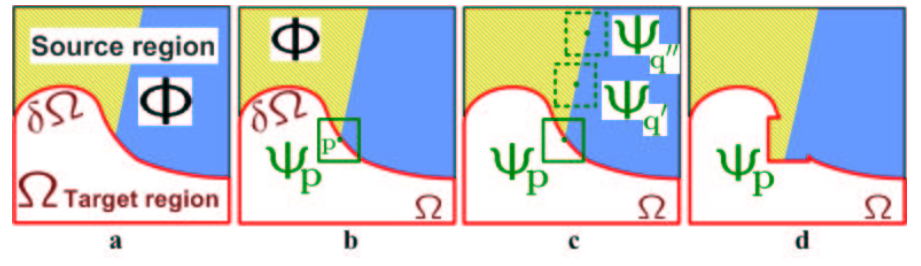
\includegraphics[scale=0.4]{Chapter3/Figures/Exemplar-based-criminisi.png}
\caption[Exemplar inpainting]{(a) Original image with target region $\Omega$, source region $\Phi$ and the contour or ``fill front'' $\delta \Omega$. (b-c) The goal is to synthesize the patch area defined by $\Psi_{p}$, using the most likely candidate ($\Psi_{q'}, \Psi_{q''}$). (d) Filling region $\Psi_{p}$ using the best matching candidate and evolving the fill front inward. This figure was taken from Criminisi~et al.\,\cite{criminisi2003object}}
\label{fig:exemplar-based}
\end{figure}

Considering the source region as the entire image minus the target region ($\Phi = I - \Omega$) and choosing a specific size of the template, all the border points are given a priority order, so that their patch region can be filled with the most similar patch from the source region.
The priority order is based on the so-called confidence term $C(p)$ and the data term $D(p)$:
\begin{subequations}
\begin{align}
P(p) & = C(p)D(p),\\
D(p) & = \vert \nabla I_{p}^{\bot}.n_{p} \vert /\alpha,\\
C(p) & = \frac{\sum\limits_{q\in\Psi_{p} \cap \Omega }C(p)}{\vert \Psi_{p}\vert},
\end{align}
\end{subequations}
\noindent where $|\Psi_{p}|$ is the area of $\Psi_{p}$, $\alpha$ is the normalization factor, $n_{p}$ is the unit vector orthogonal to the fill front ($\delta\Omega$) at point $p$, and $\nabla I_{p}^{\bot}$ illustrates the direction and intensity at this point.
After prioritizing the pixels on the border, each patch is replaced by a patch from the source region most similar to it.
The distance between two patches is based on the sum of square differences of pixels already filled in the two patches.

Fig.~\ref{fig:HairRemoval} shows some results of applying our hair removal algorithm with the default parameters.
As shown in Fig.~\ref{fig:fc} and \ref{fig:fg}, the algorithm may not be optimal if the mask detected in the first stage is not optimal.
In such cases, the optional morphological operations at the last stage of the hair detection algorithm could be removed or the default parameters adjusted.
%Since hair detection was not in the main scope of this thesis, and due to the lack of ground truth for body hair, at this point we do not have quantitative results supporting our algorithm.

\begin{figure}
\begin{center}
\subfloat[Original ]{\label{fig:fa}
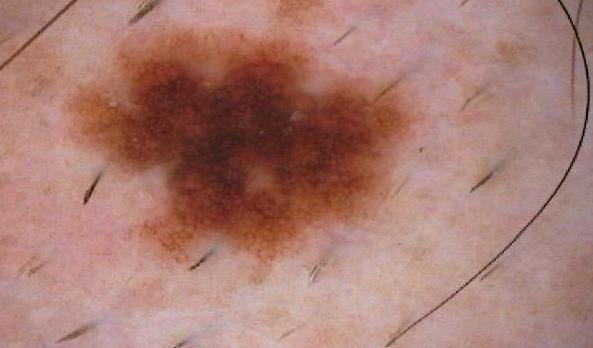
\includegraphics[width = 0.45\textwidth]{Chapter3/Figures/E1_WH_Vienna.jpg}}\
\subfloat[Restored ]{\label{fig:fb}
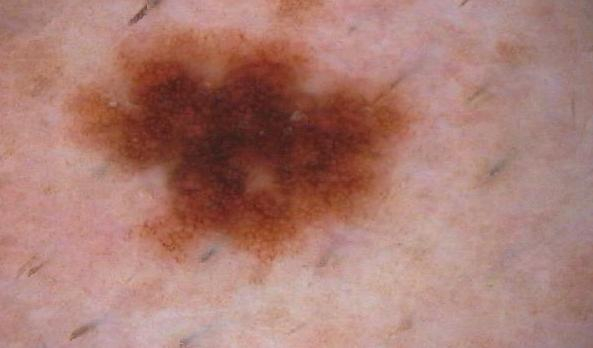
\includegraphics[width = 0.45\textwidth]{Chapter3/Figures/E1_NH_Vienna.jpg}}\\
\subfloat[Original ]{\label{fig:fc}
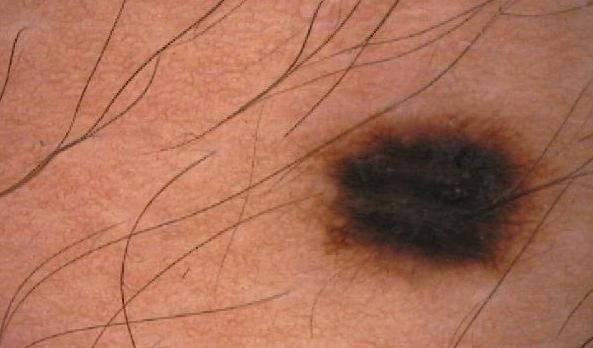
\includegraphics[width = 0.45\textwidth]{Chapter3/Figures/E4_WH_Vienna.jpg}}\
\subfloat[Restored ]{\label{fig:fd}
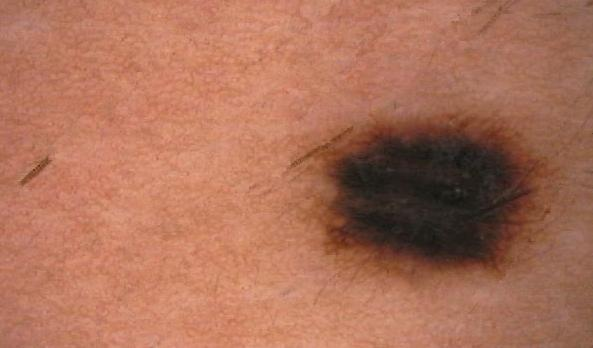
\includegraphics[width = 0.45\textwidth]{Chapter3/Figures/E4_NH_Vienna.jpg}}\\
\subfloat[Original ]{\label{fig:fe}
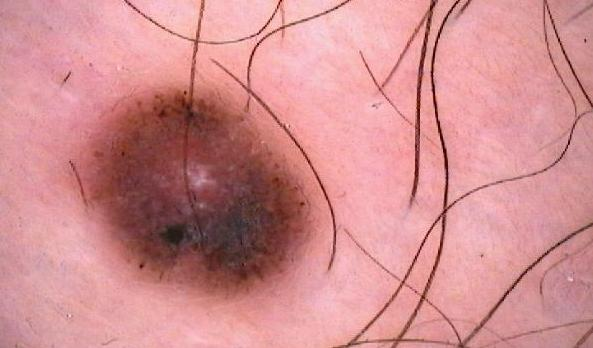
\includegraphics[width = 0.45\textwidth]{Chapter3/Figures/E5_WH_Vienna.jpg}}\
\subfloat[Restored ]{\label{fig:ff}
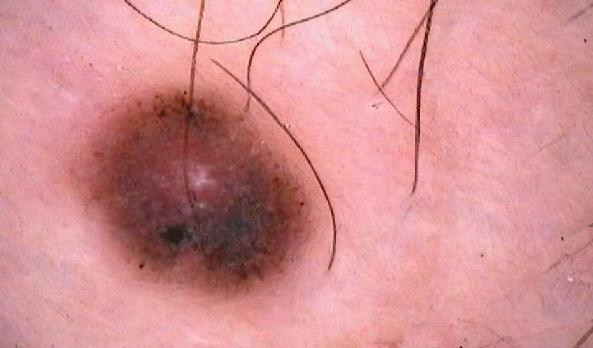
\includegraphics[width = 0.45\textwidth]{Chapter3/Figures/E5_NH_Vienna.jpg}}\\
\subfloat[Original ]{\label{fig:fg}
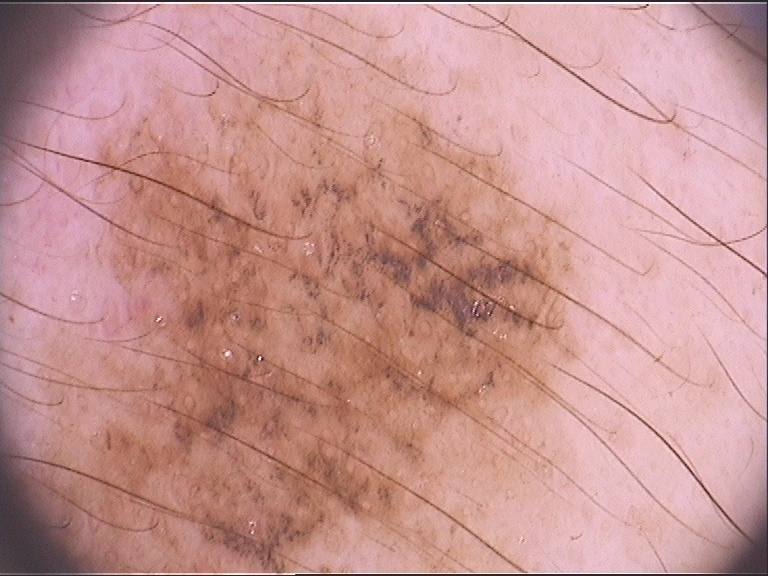
\includegraphics[width = 0.45\textwidth]{Chapter3/Figures/E1_WH_PH2.png}}\
\subfloat[Restored ]{\label{fig:fh}
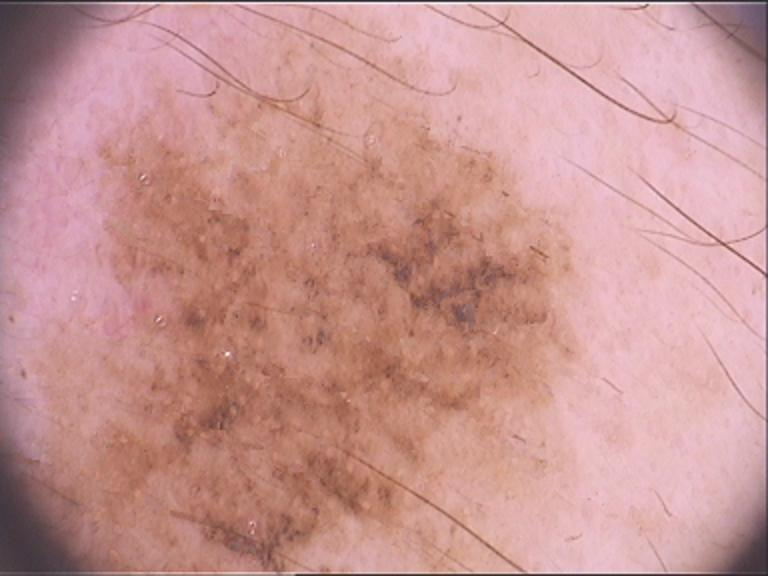
\includegraphics[width = 0.45\textwidth]{Chapter3/Figures/E1_NH_PH2.jpg}}
\end{center}
\caption[Results for the proposed hair removal algorithm]{Sample results of applying the proposed hair removal algorithm. The algorithm was used with default values for all the images. Images (a, c, e) are from the Vienna dataset and the last image (g) is from the PH$^{2}$ dataset.} %The original images are shown on the left, the images after hair removal or on the right. 

\label{fig:HairRemoval}
\end{figure}

\subsubsection{Segmentation}\label{chp3-subsubsecSeg}
A summary of segmentation and border delineation methods of pigmented skin lesions was discussed in Sect.~\ref{sec:chp2-sec2}.
In this research, a fusion of a region-based and intensity-based segmentation methods is proposed.
Our segmentation fusion is based on a region-based level-set method proposed by \cite{li2011level}, \acf{fcm}~\cite{bezdek1984fcm}, and a \acf{pdf}-based method.

%This part of the framework was proposed based on our observation and obtained results on Vienna dataset.
%The vienna dataset is a very challenging dataset for border delineation, due to illumination variations of the images. 
%Considering this dataset, without applying illumination corrections, our first approach was solely based on \ac{pdf}-based method.
%Using this initial approach we were able to correctly segment 95.428$\%$ of the dataset (corresponding to 5093 out of 5337 images).
%Forty three images were excluded, due to some severe cases of saturation or low contrast.
%However after fusion approach of level-set, \ac{pdf}-based, and \ac{fcm} algorithm, the proposed fusion method was able to segment 5310 images out of 5337 cases (corresponding to 99.49$\%$).

This part of the framework was developed using the Vienna dataset, which is very challenging for border delineation due to image illumination variations. 
Without applying any illumination corrections, our first approach used a \ac{pdf}-based method.
We were able to correctly segment 95.428$\%$ of the dataset (corresponding to 5093 out of 5337 images).
The 43 unsegmented images were excluded due to some severe cases of saturation or low contrast.
However, after combining the level-set, \ac{pdf}-based, and \ac{fcm} algorithms, we were able to segment 5310 images out of 5337 cases (corresponding to 99.49$\%$).

In the rest of this section, first each of the aforementioned methods and finally our fusion algorithm are explained. 
\begin{description}
\item[\ac{pdf}-based] method is based on analyzing the \ac{pdf} of a gray-scale, or single-channel, image.
It uses the assumption that the lesions appear in darker colors in comparison with the skin, thus they have a separate intensity profile towards the darker side of the histogram.
Based on this assumption, a Gaussian mixture with two components is fitted to the \ac{pdf} of the image, and the local minimum separating the two Gaussians is selected as the optimal threshold.
The local minimum is determined by finding the peaks of the smoothed \ac{pdf}\footnote{The \ac{pdf} is smoothed using cubic interpolation.}.
Due to illumination variations in the images, the \ac{pdf} often does not consist of a Gaussian distribution, and hence, does not have a local minimum. 
In such cases, the algorithm considers a default threshold, which can be determined empirically.  

In this study, it was observed via empirical validation that the \textit{CIE XYZ} color space was the most suitable channel for lesion segmentation.
Figure.~\ref{fig:pdfseg-b} shows the \ac{pdf} of the $Z$-channel where the first Gaussian corresponds to the pixel intensities of the lesion and the second Gaussian corresponds to the pixel intensities belonging to the skin.

Thus, as mentioned before, finding the valley between these two Gaussian bells allows us to separate the lesion from the skin (see Fig.~\ref{fig:pdfseg-a}). 
%% Figure2

\begin{figure}
	\centering
	\hspace*{\fill}
	%\subfigure[]{\label{fig:graylesion}\includegraphics[width=0.22\textwidth]{GrayLevel_D606.eps}}
	%\subfigure[]{\label{fig:grayhist}\includegraphics[width=0.22\textwidth]{GrayHist_D606.eps}}
	\subfloat[Lesion appearance of the \textit{Z} channel. The white delineation corresponds to our segmentation results.]{\label{fig:pdfseg-a}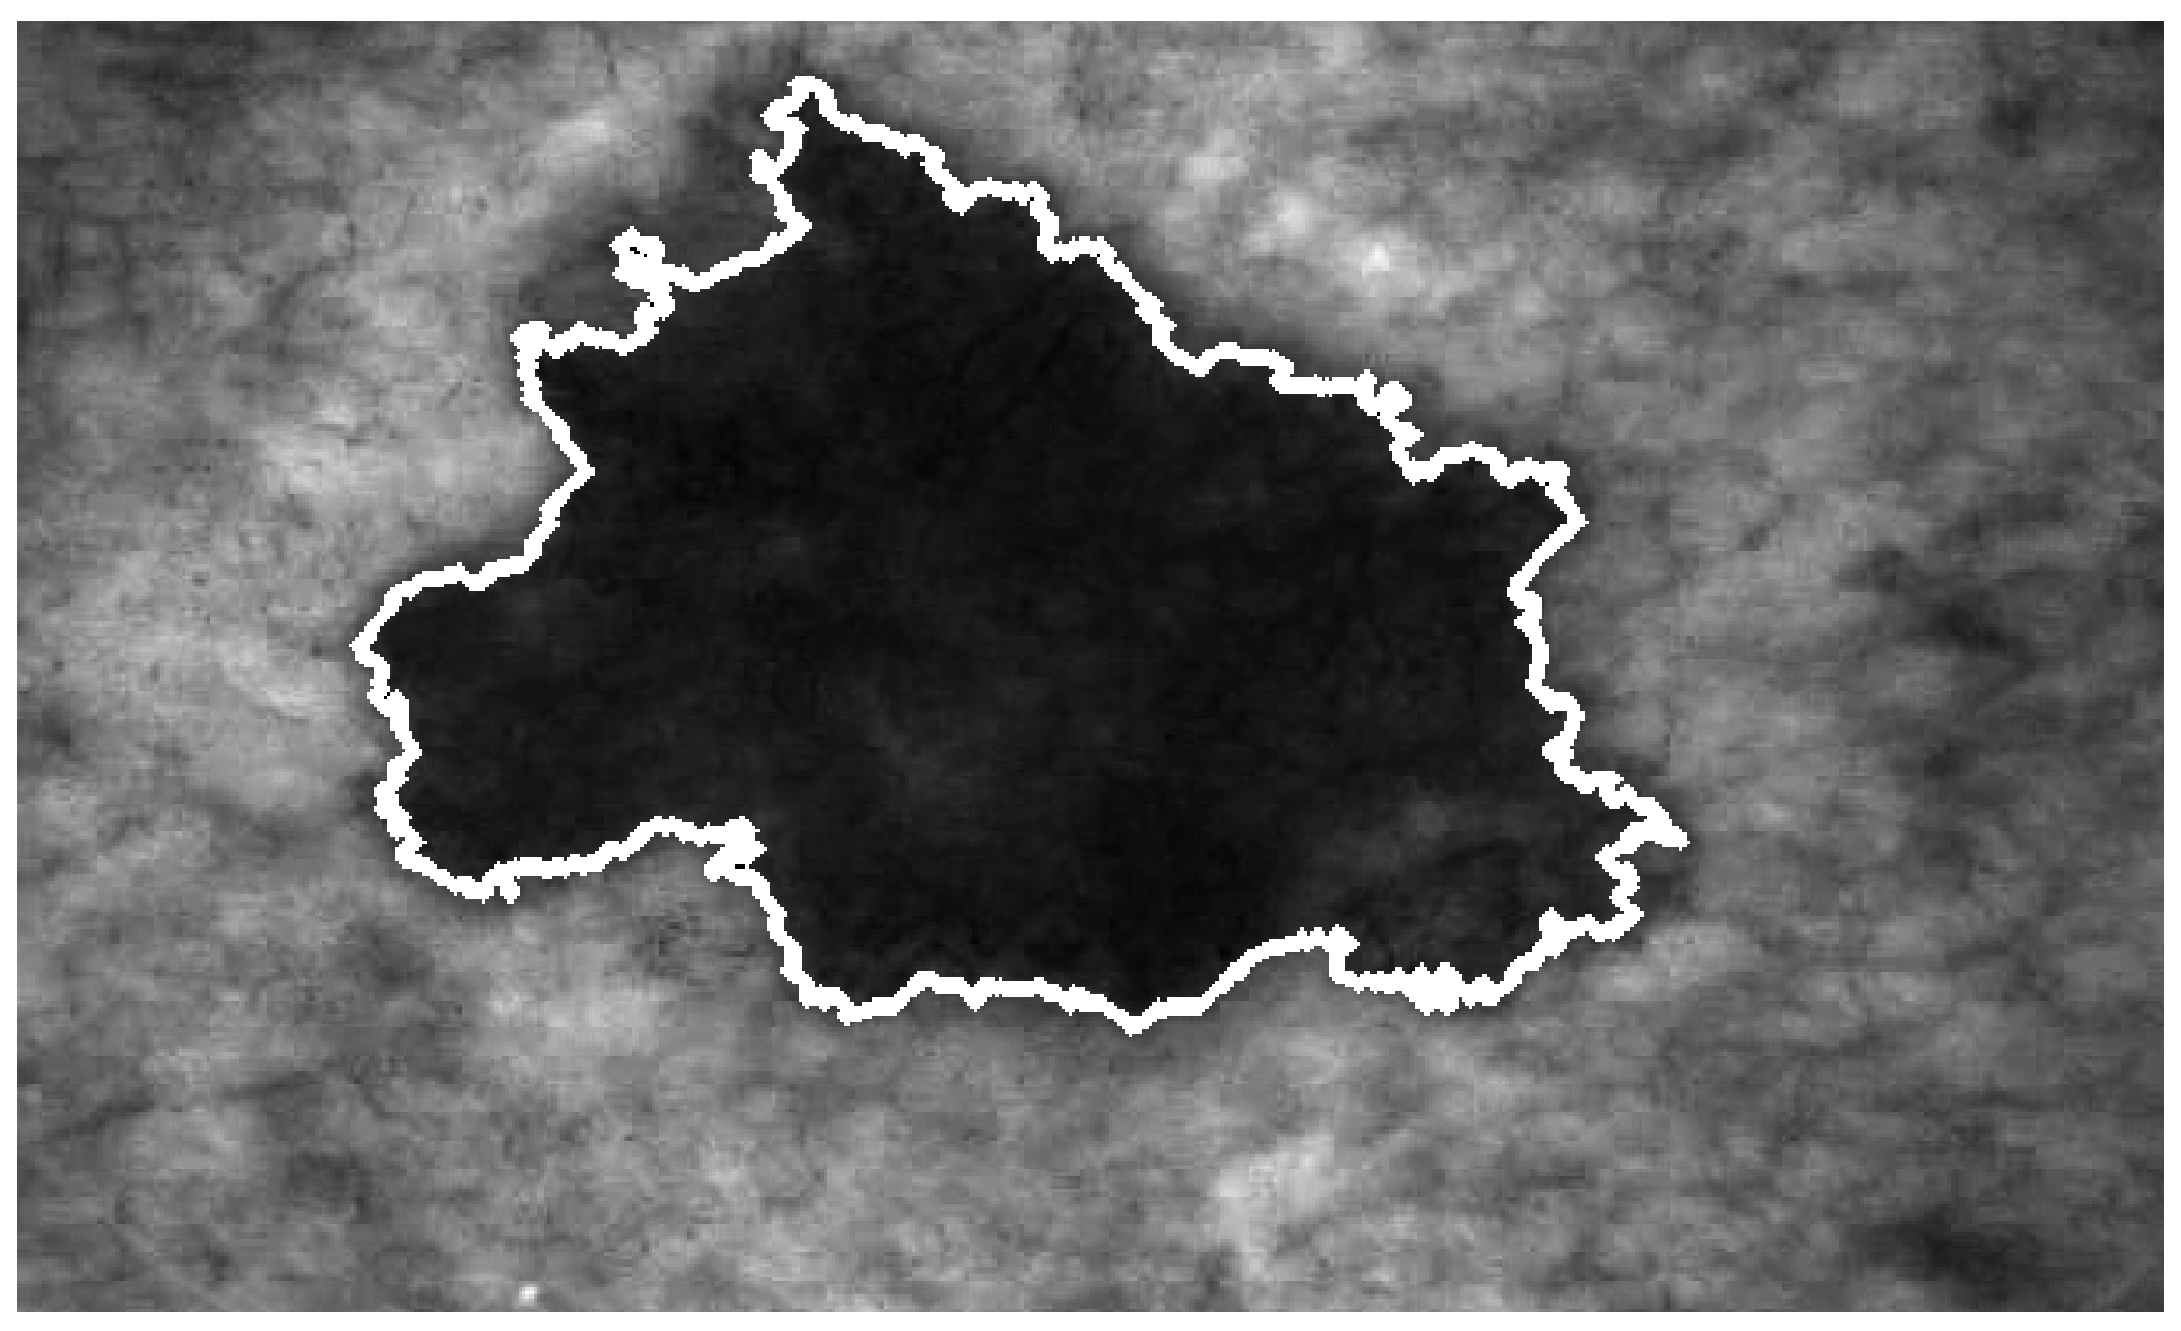
\includegraphics[height = 0.17\textheight, width=0.40\textwidth]{Chapter3/Figures/lesion_border.eps}}
	\hfill
	\subfloat[The \ac{pdf} corresponding to Fig \ref{fig:pdfseg-a}.]{\label{fig:pdfseg-b}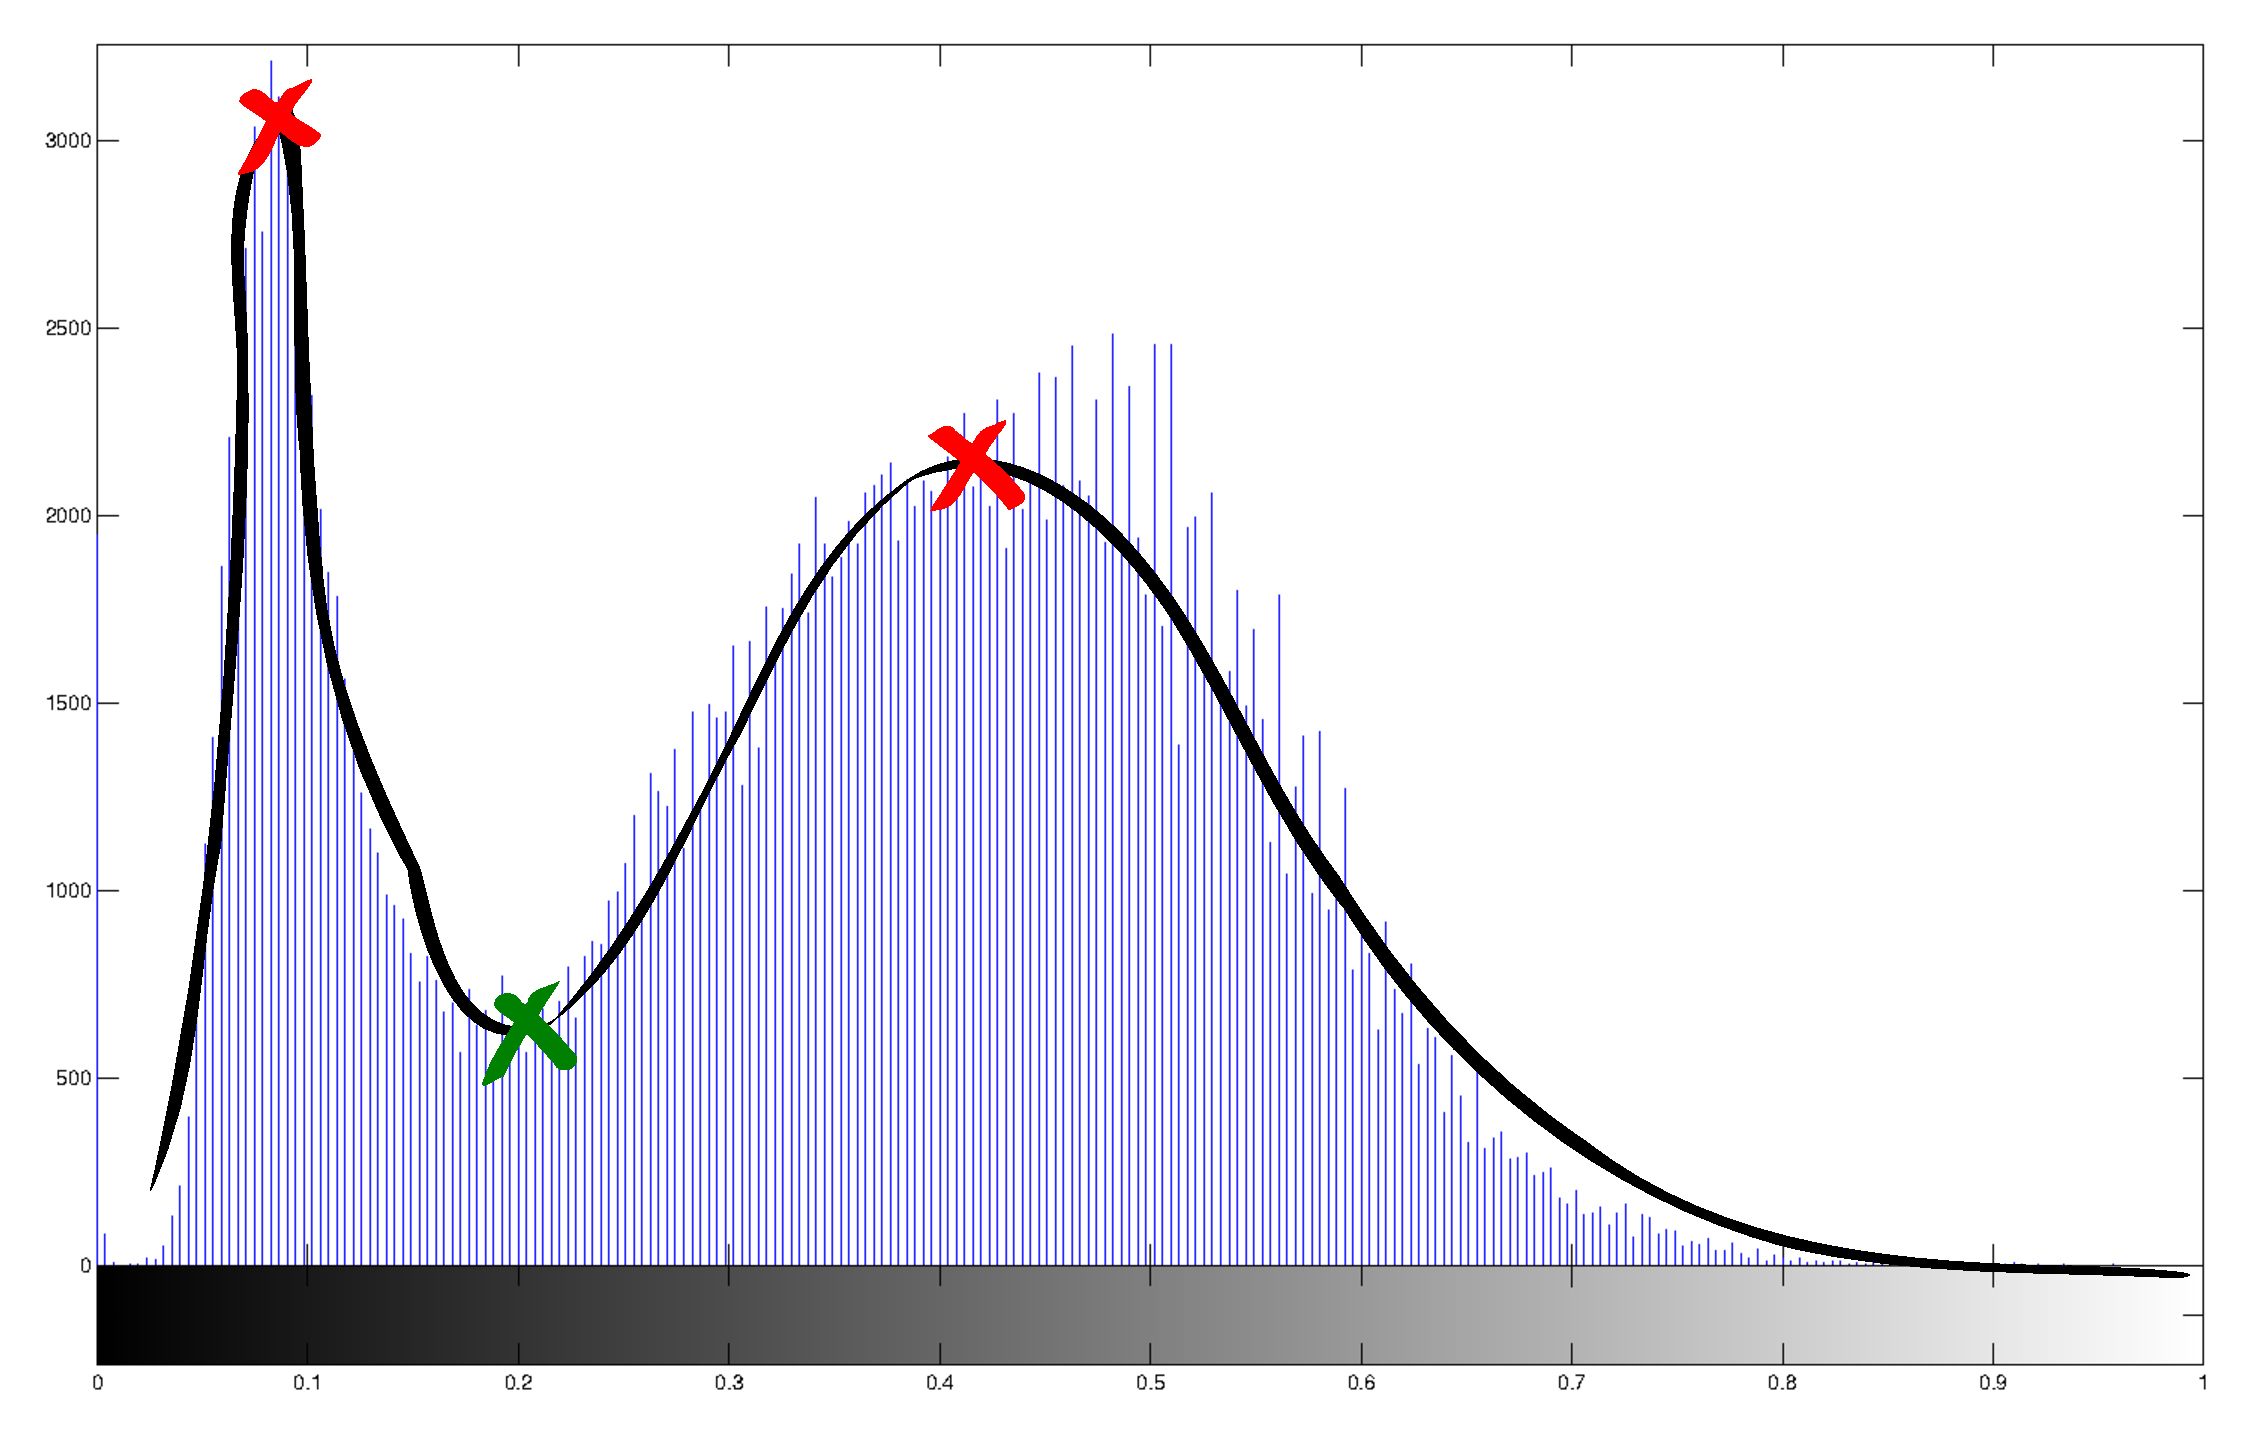
\includegraphics[ height = 0.17\textheight, width=0.40\textwidth]{Chapter3/Figures/ZNomrHist.eps}}
	\hspace*{\fill}
	\caption[\acl{pdf}-based segmentation]{Illustration of the \textit{Z} component (\textit{CIE XYZ} color space) of a dermoscopic image (a) with its corresponding \ac{pdf} (b). The distribution is characterized by a Gaussian mixture with two components. The best threshold is located at the valley between the two Gaussian bells (red cross between the the peaks).
The threshold in this case was found through the peak detetion algorithm and finding the local minium value.}
	\label{fig:pdfseg}
\end{figure}

\noindent Here, the default threshold, considering the utilization of the $Z$-channel, was set to 0.2.
Some results obtained by this algorithm are shown in the second column of Fig.~\ref{fig:plf}.
The lesions in Figs.~\ref{fig:S1a} and~\ref{fig:S1b} are under-segmented, while the lesion in Fig.~\ref{fig:S1d} is over-segmented.
However, the lesions in Figs.~\ref{fig:S1c} and~\ref{fig:S1e} are perfectly delineated.

\item[Level-set methods] are based on the general principle of the active contour, or snakes, approaches~\cite{kass1988snakes}.
These methods looks for a contour of an object by minimizing an energy function, which either uses edge information or region descriptor information.
The level-set method proposed in \cite{li2011level} is region-based because it uses region descriptor as a criterion to guide the motion of the active contour.
If the image domain is illustrated by $\Omega$, the goal of the proposed method is to find a contour $C$, which divides the image into disjoined regions $\{$ $\Omega_{1}, \Omega_{2},..., \Omega_{N}$ $\}$.
The chosen level-set method is suited to our application because it deals with intensity inhomogeneities.
This model defines a local clustering criterion function for the intensities in a circular neighborhood ($\mathcal{O}_{y}$) of each point based on two assumptions: 
(i) the bias image which accounts for intensity inhomogeneities ($b$) is changing slowly and can be approximated by a constant in a neighborhood of each point;
(ii) the pure image without inhomogeneities and noise takes approximately N distinct constant values, $c_{1}, ..., c_{N}$ for N disjoined regions $\Omega_{1}:\Omega_{N}$~\cite{li2011level}.
Based on these assumptions the local clustering criterion function is defined as: 
\begin{equation}
\mathcal{E}_{y} = \sum\limits_{i=1}^{N}\int\limits_{\Omega_{i}} K(y-x)\vert I(x)-b(y)c_{i} \vert^{2} dx~,
\label{eq:ls-lccf}
\end{equation}
\noindent Where $K(y-x)$ is a non-negative window or kernel function equal to 0 for any point outside the neighborhood ($x \notin \mathcal{O}_{y}$).
Considering this function, the optimal partitions ($\Omega_{i}$) of the entire image are defined so that $\mathcal{E}_{y}$ is minimized for all $y$ in the image.
Subsequently, the energy function is taken as the integral of $\mathcal{E}_{y}$ with respect to $y$ in the image domain. 
For the two-phase case (binary) segmentation, the level set energy function is defined as: 
\begin{subequations}
\begin{align}
& \mathcal{E}  = \int \sum\limits_{i=1}^{N}\left( \int K(y-x)\vert I(x) - b(y)c_{i}\vert^{2} dy \right) M_{i}(\phi(x)) dx, \\
& \mathcal{E}(\phi,b,c)  = \int \sum\limits_{i=1}^{N} e_{i}(x) M_{i}(\phi(x)) dx,\\
& e_{i}(x) =  \int K(y-x)\vert I(x) - b(y)c_{i}\vert^{2} dy,\\
& e_{i}(x)  = I^{2}1_{K} - 2c_{i}I(b\ast K)+c_{i}^{2}(b^{2}\ast K).
\label{eq:ls-energy}
\end{align}
\end{subequations}

\noindent The equation above illustrates how to rewrite the energy function in a simplified manner.
The last rows indicate how $e_{i}$ can be computed: $\ast$ is a convolution operation and $1_{K} = \int K(y-x) dy$, which is equal to 1 in the entire image, except near the boundary of the image domain~\cite{li2011level} and $M$ is linked to the Heaviside function.
Using the above energy function, the final level-set formulation is represented as: 
\begin{equation}
\mathcal{F}(\phi,b,c)= \mathcal{E}(\phi,b,c) + \upsilon\mathcal{L}(\phi) + \mu\mathcal{R}(\phi),
\end{equation}
\noindent where $\mathcal{L}(\phi)$ and $\mathcal{R}(\phi)$ are the regularization terms~\cite{li2011level} (see Eq.~\ref{eq:lsLR}).
\begin{subequations}
\begin{align}
\mathcal{L}(\phi) & = \int \vert \nabla H(\phi) \vert dx, \\
\mathcal{R}(\phi) & = \int p(\vert \nabla H(\phi) \vert) dx,\\
p(s) & = (s-1)^{2}/2.
\end{align}
\label{eq:lsLR}
\end{subequations}
\noindent where, $H$ is the unit step (Heaviside) function.

In this research, an initialization region with a bounding box ($200 \times 300$) is considered positioned at center of $Z$-channel.
The $\upsilon$ is set to $0.001 \times 255^{2}$, $\sigma$ is set to 4 and $\mu$ is equal to 1.
These values were set empirically.
The second column of Fig.~\ref{fig:plf} shows some segmentation results achieved by the Level-set method.
As shown, this method segments the lesions perfectly in Fig.~\ref{fig:Oa},~\ref{fig:Ob} and \ref{fig:Od} while it fails to segment the lesions in Fig.~\ref{fig:Oc} and \ref{fig:Oe}.
The difficult and challenging illumination variation and the existing shadows along the left side of the images (Fig.~\ref{fig:Oc} and \ref{fig:Oe}) are the main reasons for the failing in the level-set algorithms.
\begin{figure}
\subfloat[Filter~1]{

\includegraphics[width=0.24\textwidth]{Chapter3/Figures/F1.png}}\hfill
%\subfloat[Filter~2]{
%
\includegraphics[width=0.24\textwidth]{Chapter3/Figures/F2.eps}}\hfill
\subfloat[Filter~2]{

\includegraphics[width=0.24\textwidth]{Chapter3/Figures/F3.png}}\hfill
\subfloat[Filter~3]{

\includegraphics[width=0.24\textwidth]{Chapter3/Figures/F4.png}}
\caption[Fusion filters]{The three main filters for discarding over-segmented and wrongly segmented results prior to fusion.}
\label{fig:segfilters}
\end{figure}

\item[\acl{fcm}] algorithm~\cite{bezdek1984fcm} is a so called soft data clustering approach.
In this technique, contrary to k-\textit{means} algorithms, each data element is described by a set of membership values, which indicate the strength of its association with each cluster.
This membership value is referred to as an association probability between data elements and clusters.
Fuzzy clustering uses these memberships to assign the elements to their closest cluster.
Considering a set of data elements, $X=\{x_{1},...,x_{n}\}$, and a list of clusters, $C= \{c_{1}, ...,c_{K}\}$, a partition matrix $W_{n\times k}= \{w_{ij} \in [0,1]\}$ is defined so that each of its elements $w_{ij}$ show the degree to which an element $x_{i}$ belongs to cluster $c_{j}$.
Thus, the \ac{fcm} intends to minimize the following cost:
\begin{subequations}
\begin{align}
& \min\limits_{c} \sum\limits_{i=1}^{n}\sum\limits_{j=1}^{K} w_{ij}^{m}\Vert x_{i}-c_{j} \Vert^{2}~,\\
& w_{ij}^{m} = \frac{1}{\sum\limits_{k=1}^{K} \left(\frac{\Vert x_{i} -c_{j} \Vert}{\Vert x_{i} -c_{k} \Vert}\right)^{2/m-1}}~,
\end{align}
\end{subequations}
\noindent The $m$ is called the fuzzifier ($m\geq 1$).
Larger values of $m$ lead to a smaller membership and thus a fuzzier clustering~\cite{bezdek1984fcm}.

In this study, we performed \ac{fcm} clustering with $K=2$, and $m = 2.0$ on the $Z$-channel of each image. 
The third column of Fig.~\ref{fig:plf} shows the segmentation results obtained with the \ac{fcm} algorithm.
This algorithm segments the lesions perfectly in Fig.~\ref{fig:Oa},~\ref{fig:Ob},~\ref{fig:Oc}, and~\ref{fig:Od}.
However, it fails to segment the last lesion in Fig.~\ref{fig:Oe}.

\item[Segmentation fusion] is considered as combining the segmented results from the three algorithms into one final result.
As shown in Fig.\,\ref{fig:plf}, each algorithm often under-segments (Fig.\,\ref{fig:S1b}), over-segments (Fig.\,\ref{fig:S1d},\,\ref{fig:S3e}) or wrongly identifies some lesions (Fig.\,\ref{fig:S2c}).

Although under-segmentation is not a problem and can be corrected by fusion methods, it is preferable to avoid over-segmented or wrongly-segmented results.
Also, the initial experiments with the Vienna dataset indicated that often only one algorithm performs correctly while the other two fail.
Thus, the majority voting or any other fusion method, such as \acs{staple}, will not perform efficiently without some preliminary filtering steps.


In this regard, some basic filtering steps are proposed to identify the wrong and over segmented results.
Three main filters are used, shown in Fig.~\ref{fig:segfilters}.
Prior to applying the filters, the images are first divided into two groups: the first group, the majority group, contains images which the lesions do not touch the borders of the images.
The second group, the minority group, contains images of larger lesions.
These lesions usually cover the entire image and are connected to the border.
Through primary observation it was concluded that the level-set algorithm segments these lesions perfectly.
Subsequently, for this group, only this algorithm is used.

While for the former group, the segmented result is multiplied to each of the filters and the number of common pixels between them are measured.
This measurement defines a connectivity index ($CI$) between each filter and a segmented result.
Thus, if the segmented results have a high $CI$ with respect to filter~1 and 2 (higher than 60\%), the result is discarded as over-segmented and if it only has a high $CI$ with respect to filter~3 (over 40\%), it is considered as a wrong segmentation.
After discarding the undesired segmentations for each image, the remaining segmentations are added together.
If one or none of the segmentation results are discarded, the final result is based on majority voting of two among all three and if two of them are discarded, the final result is equal to the remaining segmentation.

%Obviously, based on the proposed fusion algorithm, the segmentation of larger lesions which cover the entire image, will be discarded in the filtering step.
%Through the primary experiments it was observed that larger lesions were best segmented with level-set algorithm.
%Thus we considered dividing the images into two categories, the smaller lesions which belong to a larger portion of the dataset were segmented through the fusion algorithm.
%However the larger lesions segmented with level-set.
%First we divide the images into two categories, the first one contains the images of large lesions which almost cover the entire image, and the second group contains the rest of the images.
%During the experiments, it was observed that level-set performs the best for the first group, while pdf-based fails to find the best threshold.  
\end{description}



\begin{figure}
\begin{center}
\subfloat[]{\label{fig:Oa}
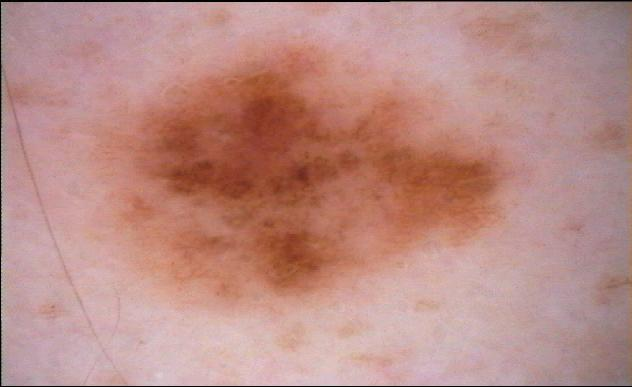
\includegraphics[scale=0.15]{Chapter3/Figures/D605.jpg}}\
\subfloat[]{\label{fig:S1a}
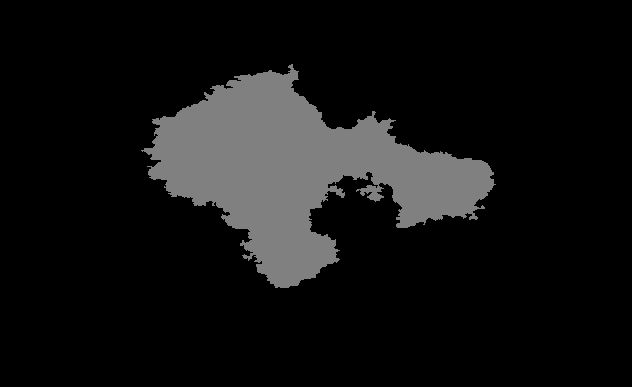
\includegraphics[scale=0.15]{Chapter3/Figures/D605-mask_pdf.png}}\
\subfloat[]{\label{fig:S2a}
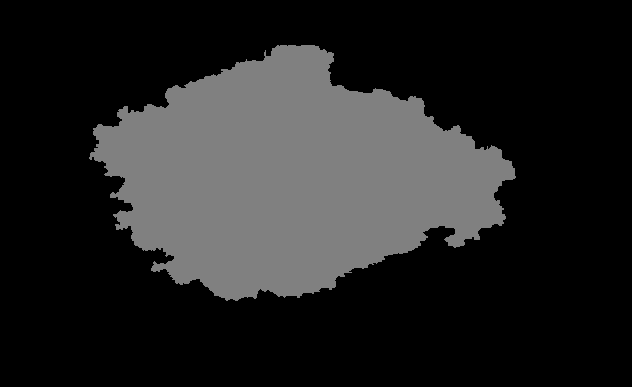
\includegraphics[scale=0.15]{Chapter3/Figures/D605-mask_LS.png}}\
\subfloat[]{\label{fig:S3a}
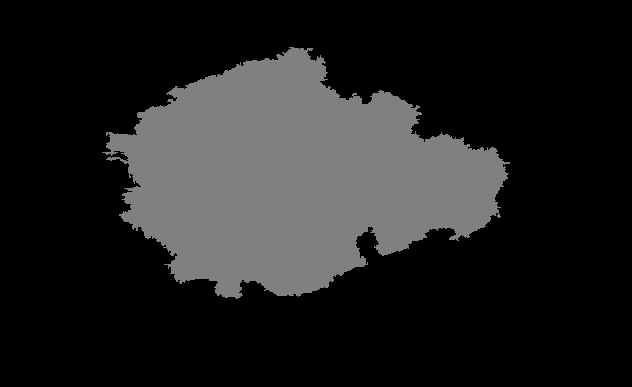
\includegraphics[scale=0.15]{Chapter3/Figures/D605-mask_FC.png}}\\
\subfloat[]{\label{fig:Ob}
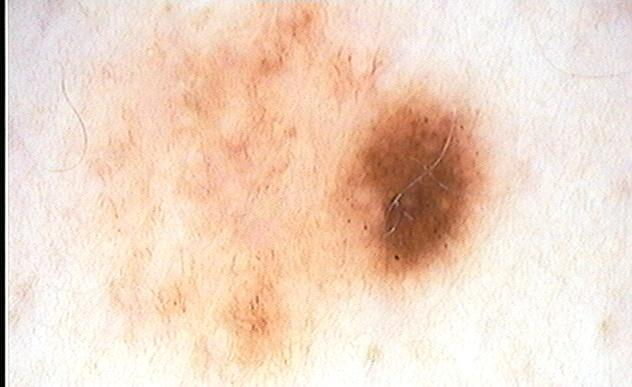
\includegraphics[scale=0.15]{Chapter3/Figures/D26.jpg}}\
\subfloat[]{\label{fig:S1b}
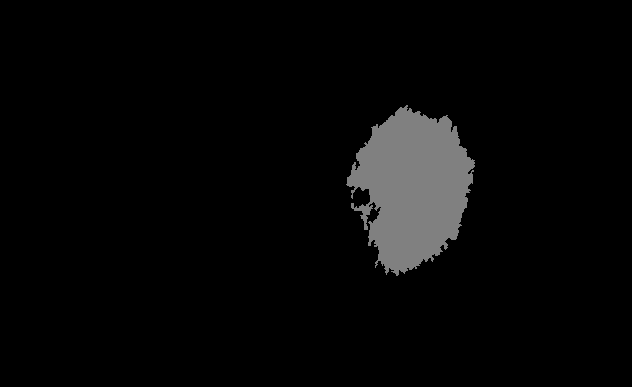
\includegraphics[scale=0.15]{Chapter3/Figures/D26-mask_pdf.png}}\
\subfloat[]{\label{fig:S2b}
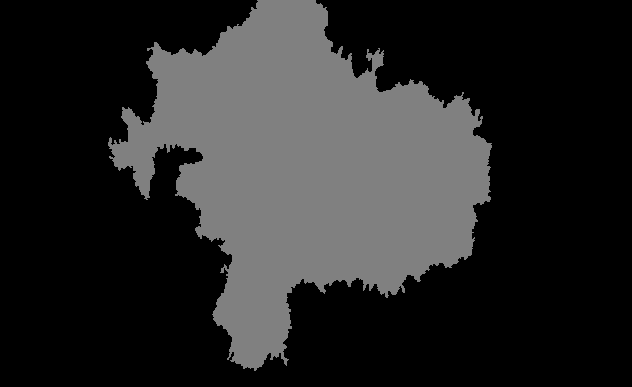
\includegraphics[scale=0.15]{Chapter3/Figures/D26-mask_LS.png}}\
\subfloat[]{\label{fig:S3b}
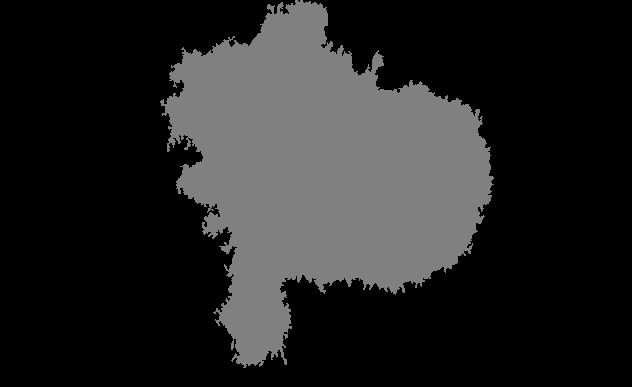
\includegraphics[scale=0.15]{Chapter3/Figures/D26-mask_FC.png}}\\
\subfloat[]{\label{fig:Oc}
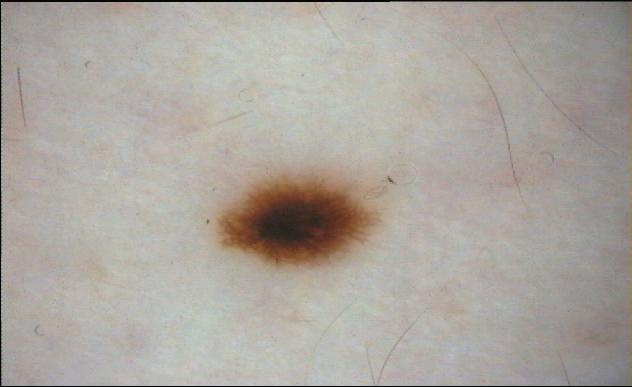
\includegraphics[scale=0.15]{Chapter3/Figures/D117.jpg}}\
\subfloat[]{\label{fig:S1c}
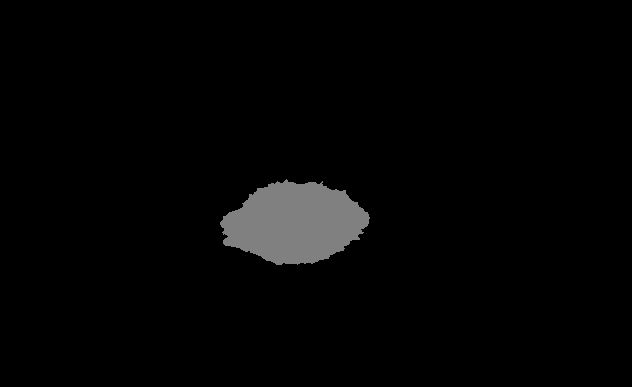
\includegraphics[scale=0.15]{Chapter3/Figures/D117-mask_pdf.png}}\
\subfloat[]{\label{fig:S2c}

\includegraphics[scale=0.15]{Chapter3/Figures/D117-mask_LS.png}}\
\subfloat[]{\label{fig:S3c}
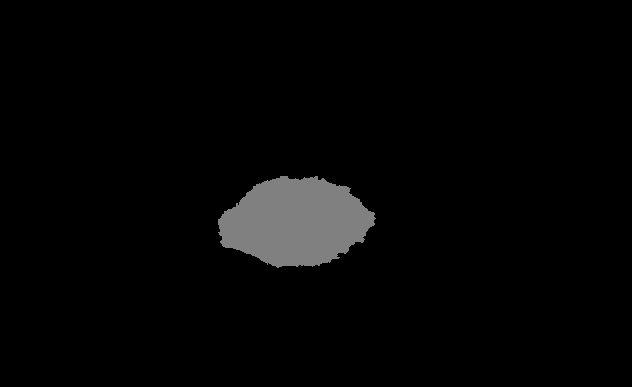
\includegraphics[scale=0.15]{Chapter3/Figures/D117-mask_FC.png}}\\
\subfloat[]{\label{fig:Od}
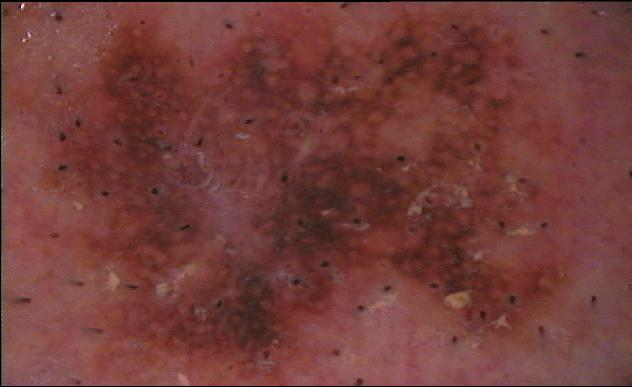
\includegraphics[scale=0.15]{Chapter3/Figures/G781.jpg}}\
\subfloat[]{\label{fig:S1d}

\includegraphics[scale=0.15]{Chapter3/Figures/G781-mask_pdf.png}}\
\subfloat[]{\label{fig:S2d}
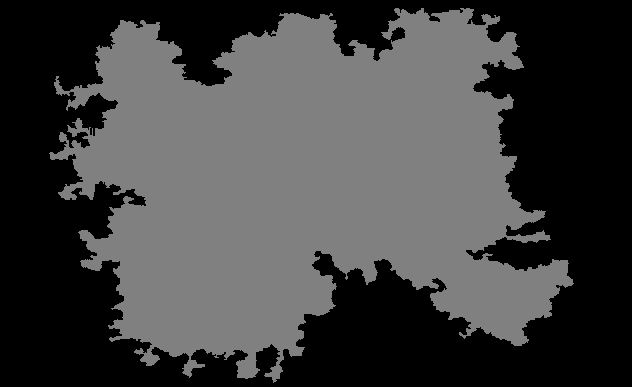
\includegraphics[scale=0.15]{Chapter3/Figures/G781-mask_LS.png}}\
\subfloat[]{\label{fig:S3d}
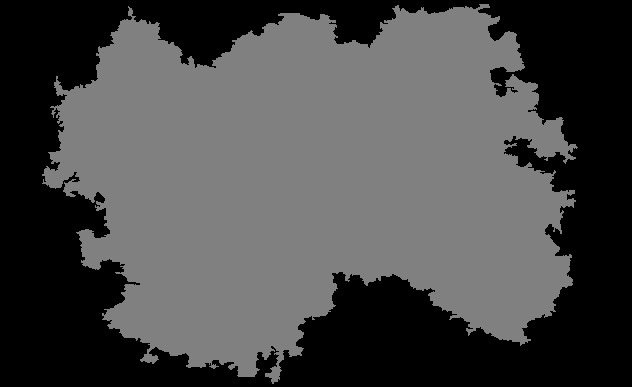
\includegraphics[scale=0.15]{Chapter3/Figures/G781-mask_FC.png}}\\
\subfloat[]{\label{fig:Oe}
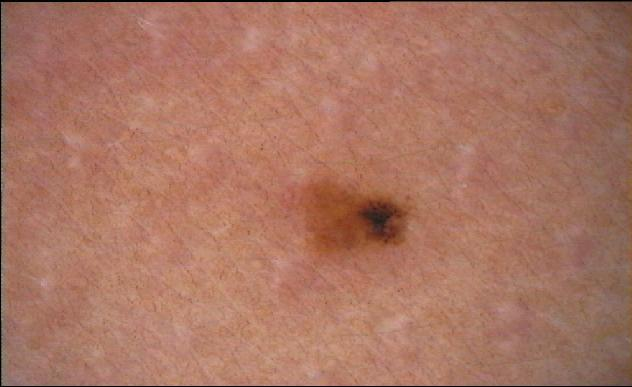
\includegraphics[scale=0.15]{Chapter3/Figures/D538.jpg}}\
\subfloat[]{\label{fig:S1e}
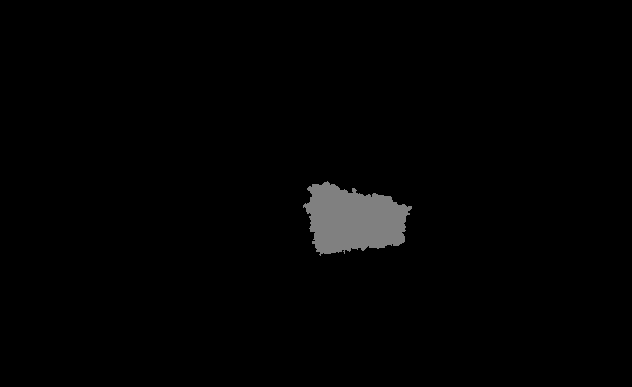
\includegraphics[scale=0.15]{Chapter3/Figures/D538-mask_pdf.png}}\
\subfloat[]{\label{fig:S2e}
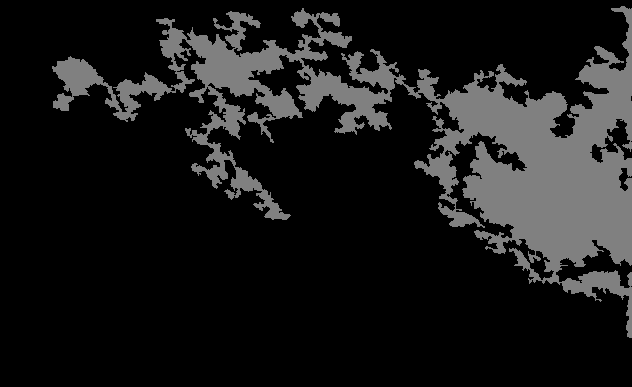
\includegraphics[scale=0.15]{Chapter3/Figures/D538-mask_LS.png}}\
\subfloat[]{\label{fig:S3e}

\includegraphics[scale=0.15]{Chapter3/Figures/D538-mask_FC.png}}\
\end{center}
\caption[Segmentation results obtained by the \ac{pdf}-based, level-set and \ac{fcm} algorithms]{Segmentation results obtained by the \ac{pdf}-based, level-set and \ac{fcm} algorithms (second, third and forth columns from the left, respectively). The original images are shown in the leftmost column.
In order to avoid the influence of the black border in the original images, the segmentation methods ignore 15 pixels along the borders of each image.
The results in rows 3--5 demonstrate the methods' failures.}
\label{fig:plf}
\end{figure} 



\subsection{Mapping}\label{chp3-subsec2}
The mapping stage is used to determine a discrete set of elements (or structures) used for the representation of each image/sample.
Therefore, two mapping strategies are defined: (i) \emph{global} and (ii) \emph{local} mapping.
In the global mapping approach, a single structure is computed for each image while in the local mapping, a set of structures is defined by sliding a window across the image.
The final descriptor is then computed based on a single element or a concatenation of elements resulting from the sliding window.
The features used to create single or multiple elements are described in the following section.

%% Table2
\begin{table}
	\footnotesize
	\caption[Extracted Features in our proposed framework]{The feature set used in this research.}
	\begin{center}
    \small
	\begin{threeparttable}
	\begin{tabular}{p{0.9\textwidth} >{\centering\arraybackslash}m{0.1\textwidth}}
	\hline \\ [-1.5ex]
	 \textbf{Feature type} & \textbf{Index} \\
	\hline \\ [-1.5ex]
	 \multicolumn{2}{l}{\textit{Shape}} \\
     \quad Thinness ratio & \multirow{4}{*}{$S$} \\
	 \quad Border asymmetry & \\
	 \quad Distance variance of border points to the center \cite{tasoulis2010skin} & \\
     \quad Statistics of gradient operator along the lesion border \cite{tasoulis2010skin} & \\ \\    
    \multicolumn{2}{l}{\textit{Color}} \\
     \quad Color variance and responses along RGB, HSI and CIELAB & \multirow{2}{*}{$C_{1}$}\\
     \quad Color histogram in RGB (\textit{b = 42} )\tnote{1} & \\
     \quad Opponent color space angle and hue histogram (\textit{b = 42}) & $C_{2}$\\ 
     \quad Color intensities & $C_{3}$\\ \\
    \multicolumn{2}{l}{\textit{Texture}} \\
	\quad Completed Local Binary Pattern\tnote{2}& $T_{1}$\\
	\quad Gray-Level Co-occurrence Matrix ($\theta$ = \{$0$, $\pi/4$, $\pi/2$, $3\pi/4$\}, \textit{D = 9 pxls}, \textit{G = 32})\tnote{3} & $T_{2}$ \\
    \quad Gabor Filter (s = 4 , $\theta$= \{$\pi/6$, $\pi/3$, $\pi/2$, $2\pi/3$, $5\pi/6$, $\pi$\}) & $T_{3}$ \\
    \quad Histogram of Oriented Gradients & $T_{4}$\\
    \quad SIFT & $T_{5}$\\ \\ [-1.5ex]
    \hline
  \end{tabular}
  \scriptsize{
  \begin{tablenotes}
  \item[1] \textit{b} stands for number of bins.
  \item[2] 24 neighbourhood, rotation invariant, uniform and normalized histogram.
  \item[3] \textit{D} stands for distance in pixels and \textit{G} is the quantized number of grey levels.
  \end{tablenotes}
  }
  \end{threeparttable}
\end{center}
\label{Tab:Table2}
\end{table}



\subsection{Feature Extraction}\label{chp3-subsec3}
Reviewing the literature, one can observe that some features are used more widely than others, such as color and shape characteristics. 
This is due to the fact that computerized systems are developed to mimic dermatologists' assessment, by using the discriminative characteristics defined in the clinical ``ABCD'' rule for instance.
Thus, we also incorporate some common shape and color descriptors along with texture features.
Shape features ($S$), color statistics and histograms ($C_{1}$), and \ac{glcm} features ($T_{2}$) are chosen because they were used widely in the past.
However, the rest of the descriptors, such as the Opponent Color Space ($C_{2}$), color intensities ($C_{3}$), \ac{lbp} ($T_{1}$), Gabor Filter ($T_{3}$), \ac{hog} ($T_{4}$), and $SIFT$ ($T_{5}$) are chosen because they are efficient and well established color and texture descriptors and have barely been used for the detection of melanoma.
These features are summarized in Table~\ref{Tab:Table2} and explained in the following.

%\input{Chapter3/Figure4.tex}	
%%\begin{table}	
%\resizebox{0.9\textwidth}{0.49\textheight}{
%    \small{
%\begin{longtable}{|p{0.24\textwidth}|p{0.5\textwidth}}
	\begin{longtable}{lc}
	\caption[Extracted features by \ac{glcm} descriptor]{The list of \ac{glcm} statistics ($f_{1}$--$f_{22}$)~\cite{haralick1973textural,clausi2002analysis,soh1999texture} used in our experiments.
	The first section of the table represents the primary measures derived from the co-occurrence matrix $C_{ij}$ for calculating the features.
	Here, $\mu_{x}$, $\mu_{y}$, $\sigma_{x}$, and $\sigma_{y}$ are the mean and standard deviation of $C_{ij}$ with respect to $i$ and $j$, respectively.
	$H_{x}$ and $H_{y}$ are entropy of $C_{x}$ and $C_{y}$}\\
%\begin{center}	
	\toprule
	Co-occurrence matrix & $C_{ij} = P_{ij}/\sum_{i,j=1}^{G} P_{ij}$\\
	& \\[-0.8ex]	
	$C_{x}(i)$ & $\sum_{j=1}^{G}C_{ij}$\\
	& \\[-0.8ex]	
	$C_{y}(j)$ & $\sum_{i=1}^{G}C_{ij}$\\
	& \\[-0.8ex]	
	$C_{x+y}(k)$ & $\sum_{{ij}_{i+j=k}} C_{ij}, k = 2,3 , 2G$ \\
	& \\[-0.8ex]	
	$C_{x-y}(k)$ & $\sum_{{ij}_{|i-j|=k}} C_{ij}, k = 0,1 , G-1$ \\	
	& \\[-0.8ex]	
	$H_{xy}$ & $-\sum_{ij}C_{ij}\log C_{ij}$ \\	
	& \\[-0.8ex]	
	$H_{xy1}$ & $-\sum_{ij}C_{ij}\log(C_{x}(i)C_{y}(j))$\\
	& \\[-0.8ex]	
	$H_{xy2}$ & $-\sum_{ij}C_{x}(i)C_{y}(j)\log(C_{x}(i)C_{y}(j))$\\
	& \\[-0.8ex]	
	\hdashline	
	& \\[-0.8ex]		
	$f_{1}$: Maximum probability & $\max\{C_{ij} , \forall (ij)\}$ \\
	& \\[-0.8ex]
	$f_{2}$: Uniformity & $\sum_{ij} C_{ij}^{2}$ \\
	& \\[-0.8ex]
	$f_{3}$: Entropy & $\sum_{ij}C_{ij}\log C_{ij}$\\
	& \\[-0.8ex]
	$f_{4}$: Dissimilarity & $\sum_{ij} C_{ij}|i-j|$\\
	& \\[-0.8ex]
	$f_{5}$: Contrast & $\sum_{ij}C_{ij}|i-j|^{2}$ \\
	& \\[-1ex]
	$f_{6}$: Inverse difference & $\sum_{ij}C_{ij}/(1+|i-j|)$ \\
	&  \\[-1ex]
	$f_{7}$: Inverse difference moment & $\sum_{ij}C_{ij}/(1+|i-j|^{2})$ \\
	
%	\hline
%	\pagebreak
%	\hline
	& \\[-1ex]
	$f_{8}$: Correlation~1 & $\sum_{ij}(i-\mu_{x})(j-\mu_{y})C_{ij}/(\sigma_{x}\sigma_{y})$\\
	& \\[-1ex] 	
	$f_{9}$: Inverse difference normalized & $\sum_{ij}C_{ij}/(1+|i-j|/N)$\\
	& \\[-1ex]
	$f_{10}$: Sum of squares & $\sum_{ij} (i-\mu)^{2}C_{ij}$ \\
	& \\[-1ex]				
	$f_{11}$: Inverse difference moment normalized & $\sum_{ij}C_{ij}/(1+|i-j|^{2}/N^{2})$\\
	& \\[-1ex]
	$f_{12}$: Sum of average & $\sum_{i=1}^{2N-1}(i+1)C_{x+y}(i)$\\
	& \\[-1ex]
	$f_{13}$: Sum entropy & $S_{e} = -\sum_{i=1}^{2N-1}C_{x+y}(i)\log C_{x+y}(i)$\\
	& \\[-1ex]
	$f_{14}$: Sum variance & $\sum_{i=1}^{2N-1}(i+1-S_{e})^{2}C_{x+y}(i)$\\
	& \\[-1ex]
	$f_{15}$: Difference variance & $\sum_{i=1}^{2N-1}i^{2}C_{x-y}(i+1)$\\
	& \\[-1ex]
	$f_{16}$: Difference entropy & $-\sum_{i=1}^{2N-1} C_{x-y}(i+1)\log C_{x-y}(i)$\\
	& \\[-1ex]
	$f_{17}$: Information measure of correlation~1 & $H_{xy}-H_{xy1}/\max(H_{x},H_{y})$ \\
	& \\[-1ex]
	$f_{18}$: Information measure of correlation~2 & $\sqrt{1-e^{-2(H_{xy2}-H_{xy})}}$\\
	& \\[-1ex]
	$f_{19}$: Auto correlation & $C = \sum_{ij}ijC_{ij}$\\
	& \\[-1ex]	
%	\hline
%	\pagebreak
%	\hline
	$f_{20}$: Correlation~2 &  $(AC-\mu_{x}\mu_{y})/\sigma_{x}\sigma_{y}$ \\
	& \\[-1ex]	
	$f_{21}$: Cluster shade & $\sum_{ij} (i+j-\mu_{x}-\mu_{y})^{3}C_{ij}$\\
	& \\[-1ex]	
	$f_{22}$: Cluster prominence & $\sum_{ij} (i+j-\mu_{x}-\mu_{y})^{4}C_{ij}$\\
	\bottomrule
	\label{tab:glcmfeatures}
  	\end{longtable}
%}
%    }
%	\end{center}
%\label{Tab:glcmfeatures}
%\end{table}

\begin{description}
\item[Shape ($S$)] features were created with reference to \cite{maglogiannis2009overview}.
This group of descriptors measures the thinness ratio, border asymmetry, distance variance of border points to the center and statistics (minimum, maximum, average and variance) of the gradient operator along the lesion's border.
	The thinness ratio measures the circularity of a lesion: $TR = 4\pi Area / Perimeter^2$. 
	And border asymmetry computes the percent of non-overlapping areas after a hypothetical folding of the lesion around its greatest diameter. 
\item[Color Variance and Color Histogram ($C_{1}$)] is a feature descriptor that has been widely used in the past for the detection of melanoma.
This descriptor contains the mean and variance of nine color channels ($R,G,B, H,S,V, L^*,a^*,b^*$) and histograms for $R$, $G$ and $B$ channels.
Each histogram is constructed with $42$ bins, leading to a final descriptor of size $(9\times2)+(42\times3) = 144$.
\end{description}
\begin{description}
\item[Opponent Color Space Angle and Hue Histogram ($C_{2}$)] were first proposed in \cite{van2006coloring} as local color features.
These descriptors were chosen due to their robustness to photometric (shadow, shading, specularities and changes of the light source) and geometrical (viewpoint, zoom and object orientation) variation.
These rotation invariant and robust descriptors are derived from $RGB$ channels using the following equations: 

\begin{subequations}
\begin{align}
	\begin{pmatrix}
	\mathcal{O}_{1}\\\mathcal{O}_{2} \\\mathcal{O}_{3}
	\end{pmatrix} & =
	\begin{pmatrix}
	(R-G)/\sqrt{2}\\
	(R+G-2B)/\sqrt{6}\\
	(R+G+B)/\sqrt{3}
	\end{pmatrix}~, \label{eq:opponent}\\	 
	H^{\mathcal{O}} & = \arctan\left(\frac{\sqrt{3}(R-G)}{R+G-2B}\right)~,\\
	\theta_{d}^{\mathcal{O}} & = \arctan\left(\frac{\sqrt{3}(R'_{d}-G'_{d})}{R'_{d}+G'_{d}-2B'_{d}}\right)~,	
\end{align}
\label{eq:HueOppAngle}
\end{subequations}	
\noindent Here $d$ denotes the spatial coordinates of ($x$,$y$) and $R'_{d}$, $G'_{d}$, $B'_{d}$ denote the first order derivatives of $RGB$ with respect to the coordinates.
This color descriptor is built by taking a 42 bins histogram for the opponent angle $\theta^{O}_{d}$ and the hue channel $H^{\mathcal{O}}$, for a final descriptor size of 84 dimensions.

%\item[Color intensities ($C_{3}$)] represent the color information in a simplest form, their intensities.
\item[Color intensities ($C_{3}$)] represent the color information in its simplest form---their intensities.
This descriptor concatenates color intensities in $R$, $G$ and $B$ to create a feature descriptor.
\item[\acf{clbp} ($T_{1}$)] is a discriminative rotation invariant feature descriptor proposed by Guo~et al.~\cite{guo2010completed}.
\ac{clbp} is a completed version of \ac{lbp}~\cite{ojala2002multiresolution}, especially designed for texture classification.
In both descriptors, a central pixel ($g_c$) in a neighborhood defined by radius $R$ is compared to its neighborhood pixels ($g_{p}$, at distance $R$ from the central pixel) and their differences are encoded in terms of binary patterns.
The binary patterns are calculated for each pixel in a given image and their histogram defines the final descriptor.
\newcounter{row}
\newcounter{col}
\newcommand\setrow[3]{
  \setcounter{col}{1}
  \foreach \n in {#1, #2, #3} {
    \edef\x{\value{col} - 0.5}
    \edef\y{3.5 - \value{row}}
    \node[anchor=center] at (\x, \y) {\n};
    \stepcounter{col}
  }
  \stepcounter{row}
}

%  
\tikzstyle{module}=[draw, draw=blue!80, text width=10em, 
    text centered, minimum height=5em, minimum width = 15em, drop shadow, rounded corners,
    fill=blue!30]
    
\tikzstyle{block} = [rectangle, draw, fill=blue!30, 
     text width=5em,text centered, rounded corners, minimum height=4em, minimum width = 5em]
\tikzstyle{block1} = [rectangle, draw, fill=white!20, 
     text width=5em,text centered, rounded corners, minimum height=4em, minimum width = 5em]

\tikzstyle{line} = [draw, -latex']

% Define distances for bordering
\def\blockdist{1}
\def\edgedist{1.5}
  
\begin{figure}			
\begin{center}
\subfloat[]{
\scalefont{0.7}
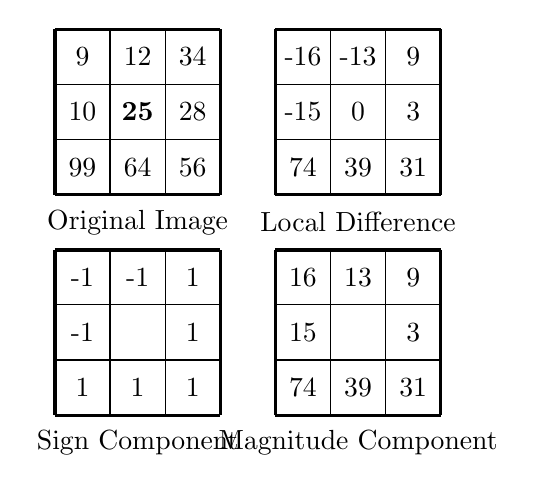
\begin{tikzpicture}[scale=.7]

  \begin{scope}
    \draw (0, 0) grid (3, 3);
    \draw[very thick, scale=3] (0, 0) grid (1, 1);

    \setcounter{row}{1}
    \setrow {9}{12}{34} 
    \setrow {10}{\textbf{25}}{28}  
    \setrow {99}{64}{56}  
    \node[anchor=center] at (1.5, -0.5) {Original Image};
  \end{scope}

  \begin{scope}[xshift=4cm]
    \draw (0, 0) grid (3,3);
    \draw[very thick, scale=3] (0, 0) grid (1,1);

    \setcounter{row}{1}
    \setrow {-16}{-13}{9}  
    \setrow {-15}{0}{3}  
    \setrow {74}{39}{31} 
    \node[anchor=center] at (1.5, -0.5) {Local Difference};
  \end{scope}

  \begin{scope}[yshift=-4cm]
    \draw (0, 0) grid (3,3);
    \draw[very thick, scale=3] (0, 0) grid (1,1);

    \setcounter{row}{1}
    \setrow {-1}{-1}{1}  
    \setrow {-1}{}{1}  
    \setrow {1}{1}{1} 
    \node[anchor=center] at (1.5, -0.5) {Sign Component};
  \end{scope}
  
    \begin{scope}[yshift=-4cm,xshift =4cm]
    \draw (0, 0) grid (3,3);
    \draw[very thick, scale=3] (0, 0) grid (1,1);

    \setcounter{row}{1}
    \setrow {16}{13}{9}  
    \setrow {15}{}{3}  
    \setrow {74}{39}{31} 
    \node[anchor=center] at (1.5, -0.5) {Magnitude Component};
  \end{scope}
\end{tikzpicture}
}\\
\subfloat[]{
\begin{tikzpicture}[node distance = 10cm,scale=0.7, every node/.style={scale=0.7}] % 
    % Place nodes   
\begin{scope}[node distance=10cm]
	\node[block] (CLBPs){ $CLBP_{s}$};
\end{scope}
\node[block,below of=CLBPs , node distance = 3cm] (CLBPm) { $CLBP_{m}$};
\node[block,below of=CLBPm, node distance =3cm] (CLBPc) { $CLBP_{c}$};
\node [block, left of=CLBPc, node distance =4cm] (GL) {Grey level of center};
\node [block, above of=GL, node distance =4cm] (LC) {Local Differences}; 
    
    \begin{pgfonlayer}{background}
	\path (LC.west |- LC.north)+(-0.3,-0.8+\blockdist) node (a) {};
    \path (GL.east |- GL.south)+(+0.3,-0.3) node (b) {};          
    \path[fill=blue!10,rounded corners, draw=blue!20, dashed] (a) rectangle (b);
	\end{pgfonlayer}
	
	\begin{pgfonlayer}{background}
	\path (CLBPs.west |- CLBPs.north)+(-0.3,-0.3+\blockdist) node (c) {};
    \path (CLBPc.east |- CLBPc.south)+(+0.3,-0.3) node (d) {};          
    \path[fill=blue!10,rounded corners, draw=blue!20, dashed] (c) rectangle (d);
	\end{pgfonlayer}
	\path (CLBPs.west |- CLBPs.north) +(+1.05,-0.7+\blockdist) node (bgfea) { Binary Patterns};
	
	\path (CLBPs.east |- CLBPs.north)+(0.2,-0.4+\blockdist) node (i) {};
	\path (CLBPc.east |- CLBPc.south)+(0.2,-0.4) node (j) {};

	\draw[decorate,decoration={brace,raise=6pt,amplitude=10pt}, thick]
    (i)--(j) ;
    
    	\path (CLBPs.west |- CLBPs.north)+(-0.15,0) node (k) {};
	\path (CLBPm.west |- CLBPm.south)+(-0.15,0) node (l) {};
text width=3cm
	\draw[decorate,decoration={brace,raise=6pt,amplitude=10pt, mirror}, thick]
    (k)--(l) ;
    
	%% Defining a position for the next block
	\path (CLBPm.east |- CLBPm.north)+(+0.5,-0.6) node (e) {};
	\node[block,right of=CLBPm, node distance = 4.5cm] (CLBPMap) {CLBP Map};
	\node[block,right of=CLBPMap, node distance = 3cm] (CLBPHist) {CLBP \\ Histogram};

	\path (LC.west |- LC.south)+(+0.5,-1) node (f) {};
	\node[block1,left of=f, node distance = +3cm] (Img) {Original \\ Image};
	\path (LC.west |- LC.north)+(-0.15,0) node (m) {};
	\path (GL.west |- GL.south)+(-0.15,0) node (n) {};
		\draw[decorate,decoration={brace,raise=6pt,amplitude=10pt, mirror}, thick]
    (m)--(n) ;
    
    \path [line] (CLBPMap) -- (CLBPHist);
    \path (CLBPm.east |- CLBPm.south)+(1.1,0.7) node (o) {};
    \path [line] (o)--(CLBPMap); 

\end{tikzpicture}}
\end{center}
\caption[\ac{clbp} algorithm]{\ac{clbp} descriptor process. An example of how local distances, sign and magnitude components are calculated is given in (a), while (b) shows an overall view of the CLBP process.}
\label{fig:CLBPFig}
\end{figure}

\begin{figure}
\centering
\subfloat[$\pi/6$]{

\includegraphics[scale=0.06]{Chapter3/Figures/Gabor-pi-6.png}}
\subfloat[$\pi/3$]{

\includegraphics[scale=0.06]{Chapter3/Figures/Gabor-pi-3.png}}
\subfloat[$\pi/2$]{

\includegraphics[scale=0.06]{Chapter3/Figures/Gabor-pi-2.png}}
\subfloat[$2\pi/3$]{

\includegraphics[scale=0.06]{Chapter3/Figures/Gabor-2pi-3.png}}
\subfloat[$5\pi/6$]{

\includegraphics[scale=0.06]{Chapter3/Figures/Gabor-5pi-6.png}}
\subfloat[$\pi$]{

\includegraphics[scale=0.06]{Chapter3/Figures/Gabor-pi.png}}
\caption[Six orientation of Gabor filter]{The 6 orientations of the Gabor filters.}
\label{fig:GaborOrientation}
\end{figure}
		
The local patterns of the \ac{clbp} descriptor encode the magnitude and sign differences between the central pixel and its neighbors as well as the grey level of the central pixel rather than only the sign differences (general \ac{lbp}).
Figure \ref{fig:CLBPFig} represents this process.
The sign $CLBP_S$, magnitude $CLBP_M$, and central grey level $CLBP_C$ binary patterns are created by encoding the local distance components and the central grey levels.  

In the proposed framework, the rotation invariant, uniform, and normalized \ac{clbp} features with a radius of 3 and $24$ samples were calculated.
The radius and number of samples were chosen after testing the algorithm with different neighboring samples such as $\{8, 16, 24\}$ with a radius of $\{1,2,3\}$, respectively.
\end{description}
\begin{description}
\item[\acf{glcm} ($T_{2}$)] is one of the earliest texture descriptor methods, proposed by Haralick.~et al.~\cite{haralick1973textural}, widely used for texture analysis applications, including melanoma detection.
In this approach, texture features are extracted based on the statistical measurement of co-occurrence probabilities.
The co-occurrence distribution represents the occurrence probabilities of all the pairwise combinations of the grey levels in a defined window~\cite{clausi2002analysis}.
In other words, it counts how often a pixel with the grey intensity $i$ occurs adjacent to a pixel with the grey intensity $j$.
The spatial distance and orientation of interests between the pixels are defined by the distance $D$ and the angle $\theta$.
The co-occurrence probability between grey levels $i$ and $j$ is defined in Eq.~\ref{eq:GLCM}, where $P_{ij}$ represents the conditional probability of occurrences of the grey value $i$ adjacent to the grey value $j$ given the distance $D$ and orientation $\theta$.
Here, $G$ is the quantized number of grey levels:
\begin{equation}
    C_{ij} = \frac{P_{ij}}{\sum_{i,j=1}^{G} P_{ij}}.   
\label{eq:GLCM}
\end{equation}

The images are quantized to 32 grey levels and the co-occurrence probabilities are calculated given the distance ($D$) of 9 pixels and four different orientations of \{$\theta$ = $0^{\circ}$, $45^{\circ}$, $90^{\circ}$, $135^{\circ}$\}.
The final texture descriptor is an average of these four measurements allowing us to obtain a rotation invariant descriptor.
For each orientation, a set of 22 texture features (proposed in \cite{haralick1973textural, clausi2002analysis, soh1999texture}) are calculated.
These features are listed in Table~\ref{tab:glcmfeatures}
The proposed distance and quantization values were chosen after testing a variety of distances $\{1, 3, 7, 9\}$ and quantized grey-levels $\{16, 32, 64\}$.
%\begin{table}	
%\resizebox{0.9\textwidth}{0.49\textheight}{
%    \small{
%\begin{longtable}{|p{0.24\textwidth}|p{0.5\textwidth}}
	\begin{longtable}{lc}
	\caption[Extracted features by \ac{glcm} descriptor]{The list of \ac{glcm} statistics ($f_{1}$--$f_{22}$)~\cite{haralick1973textural,clausi2002analysis,soh1999texture} used in our experiments.
	The first section of the table represents the primary measures derived from the co-occurrence matrix $C_{ij}$ for calculating the features.
	Here, $\mu_{x}$, $\mu_{y}$, $\sigma_{x}$, and $\sigma_{y}$ are the mean and standard deviation of $C_{ij}$ with respect to $i$ and $j$, respectively.
	$H_{x}$ and $H_{y}$ are entropy of $C_{x}$ and $C_{y}$}\\
%\begin{center}	
	\toprule
	Co-occurrence matrix & $C_{ij} = P_{ij}/\sum_{i,j=1}^{G} P_{ij}$\\
	& \\[-0.8ex]	
	$C_{x}(i)$ & $\sum_{j=1}^{G}C_{ij}$\\
	& \\[-0.8ex]	
	$C_{y}(j)$ & $\sum_{i=1}^{G}C_{ij}$\\
	& \\[-0.8ex]	
	$C_{x+y}(k)$ & $\sum_{{ij}_{i+j=k}} C_{ij}, k = 2,3 , 2G$ \\
	& \\[-0.8ex]	
	$C_{x-y}(k)$ & $\sum_{{ij}_{|i-j|=k}} C_{ij}, k = 0,1 , G-1$ \\	
	& \\[-0.8ex]	
	$H_{xy}$ & $-\sum_{ij}C_{ij}\log C_{ij}$ \\	
	& \\[-0.8ex]	
	$H_{xy1}$ & $-\sum_{ij}C_{ij}\log(C_{x}(i)C_{y}(j))$\\
	& \\[-0.8ex]	
	$H_{xy2}$ & $-\sum_{ij}C_{x}(i)C_{y}(j)\log(C_{x}(i)C_{y}(j))$\\
	& \\[-0.8ex]	
	\hdashline	
	& \\[-0.8ex]		
	$f_{1}$: Maximum probability & $\max\{C_{ij} , \forall (ij)\}$ \\
	& \\[-0.8ex]
	$f_{2}$: Uniformity & $\sum_{ij} C_{ij}^{2}$ \\
	& \\[-0.8ex]
	$f_{3}$: Entropy & $\sum_{ij}C_{ij}\log C_{ij}$\\
	& \\[-0.8ex]
	$f_{4}$: Dissimilarity & $\sum_{ij} C_{ij}|i-j|$\\
	& \\[-0.8ex]
	$f_{5}$: Contrast & $\sum_{ij}C_{ij}|i-j|^{2}$ \\
	& \\[-1ex]
	$f_{6}$: Inverse difference & $\sum_{ij}C_{ij}/(1+|i-j|)$ \\
	&  \\[-1ex]
	$f_{7}$: Inverse difference moment & $\sum_{ij}C_{ij}/(1+|i-j|^{2})$ \\
	
%	\hline
%	\pagebreak
%	\hline
	& \\[-1ex]
	$f_{8}$: Correlation~1 & $\sum_{ij}(i-\mu_{x})(j-\mu_{y})C_{ij}/(\sigma_{x}\sigma_{y})$\\
	& \\[-1ex] 	
	$f_{9}$: Inverse difference normalized & $\sum_{ij}C_{ij}/(1+|i-j|/N)$\\
	& \\[-1ex]
	$f_{10}$: Sum of squares & $\sum_{ij} (i-\mu)^{2}C_{ij}$ \\
	& \\[-1ex]				
	$f_{11}$: Inverse difference moment normalized & $\sum_{ij}C_{ij}/(1+|i-j|^{2}/N^{2})$\\
	& \\[-1ex]
	$f_{12}$: Sum of average & $\sum_{i=1}^{2N-1}(i+1)C_{x+y}(i)$\\
	& \\[-1ex]
	$f_{13}$: Sum entropy & $S_{e} = -\sum_{i=1}^{2N-1}C_{x+y}(i)\log C_{x+y}(i)$\\
	& \\[-1ex]
	$f_{14}$: Sum variance & $\sum_{i=1}^{2N-1}(i+1-S_{e})^{2}C_{x+y}(i)$\\
	& \\[-1ex]
	$f_{15}$: Difference variance & $\sum_{i=1}^{2N-1}i^{2}C_{x-y}(i+1)$\\
	& \\[-1ex]
	$f_{16}$: Difference entropy & $-\sum_{i=1}^{2N-1} C_{x-y}(i+1)\log C_{x-y}(i)$\\
	& \\[-1ex]
	$f_{17}$: Information measure of correlation~1 & $H_{xy}-H_{xy1}/\max(H_{x},H_{y})$ \\
	& \\[-1ex]
	$f_{18}$: Information measure of correlation~2 & $\sqrt{1-e^{-2(H_{xy2}-H_{xy})}}$\\
	& \\[-1ex]
	$f_{19}$: Auto correlation & $C = \sum_{ij}ijC_{ij}$\\
	& \\[-1ex]	
%	\hline
%	\pagebreak
%	\hline
	$f_{20}$: Correlation~2 &  $(AC-\mu_{x}\mu_{y})/\sigma_{x}\sigma_{y}$ \\
	& \\[-1ex]	
	$f_{21}$: Cluster shade & $\sum_{ij} (i+j-\mu_{x}-\mu_{y})^{3}C_{ij}$\\
	& \\[-1ex]	
	$f_{22}$: Cluster prominence & $\sum_{ij} (i+j-\mu_{x}-\mu_{y})^{4}C_{ij}$\\
	\bottomrule
	\label{tab:glcmfeatures}
  	\end{longtable}
%}
%    }
%	\end{center}
%\label{Tab:glcmfeatures}
%\end{table}

\item[Gabor Filter ($T_{3}$)] is a linear filter which extracts edges and texture information from the image and was found to be similar to human visual perception~\cite{marvcelja1980mathematical}.
	The Gabor filter is defined as a modulation of a Gaussian kernel with a sinusoidal wave.
	The Gabor expression is shown in Eq.~\ref{eq:Gabor}.
	This function is basically a Gaussian with standard deviations of $\sigma_{x}$ and $\sigma_{y}$ that vary along the $x$ and $y$ axes while it is modulated by a complex sinusoidal with a wavelength of $\lambda$.
	In this equation, $\theta$ represents the orientation of the Gabor filter, $\psi$ is the phase offset, and $s$ is the scale factor.	
	\begin{subequations}
	\begin{align}
	g(x,y) & = \exp \left(-\left(\frac{x'^2}{2\sigma_{x}^{2}}+\frac{y'^{2}}{2\sigma_{y}^{2}}\right)\right) \cos\left(2\pi\frac{x'}{\lambda}+ \psi\right), \\
	x'& = s(x\cos\theta + y\sin\theta),\\
	y' &= s(-x\sin\theta + y\cos\theta).	
	\end{align}
	\label{eq:Gabor}
	\end{subequations}
	
In this work as described by \cite{Manjunath96-45}, the images are convolved with a set of Gabor filters characterized by different orientations and scales.
The features are created by considering the mean and variance of the resulting filtering.
We used 6 different orientations (\{$\pi/6$, $\pi/3$, $\pi/2$, $2\pi/3$, $5\pi/6$, $\pi$\}) along 4 scales, downsizing by a factor of two between each scale.
The first 6 filters are shown in Fig.~\ref{fig:GaborOrientation}.
%	\begin{figure}
	%\centering
	%\subfloat[$\pi/6$]{
	%
\includegraphics[scale=0.06]{Chapter3/Figures/Gabor-pi-6.png}}
	%\subfloat[$\pi/3$]{
	%
\includegraphics[scale=0.06]{Chapter3/Figures/Gabor-pi-3.png}}
	%\subfloat[$\pi/2$]{
	%
\includegraphics[scale=0.06]{Chapter3/Figures/Gabor-pi-2.png}}
	%\subfloat[$2\pi/3$]{
	%
\includegraphics[scale=0.06]{Chapter3/Figures/Gabor-2pi-3.png}}
	%\subfloat[$5\pi/6$]{
	%
\includegraphics[scale=0.06]{Chapter3/Figures/Gabor-5pi-6.png}}
	%\subfloat[$\pi$]{
	%
\includegraphics[scale=0.06]{Chapter3/Figures/Gabor-pi.png}}
	%\caption[Six orientations of the Gabor filter]{The 6 orientations of the Gabor filter.}
	%\label{fig:GaborOrientation}
	%\end{figure}

\item[\acf{hog} ($T_{4}$)] was proposed in \cite{dalal2005histograms}.
In simple terms, \ac{hog} counts the occurrences of gradient orientations in localized patches of an image.
This descriptor is invariant to geometric and photometric transformations.
\ac{hog} calculates the gradient values of the image by applying derivative filters ($[-1,0,1]$, $[-1,0,1]^{T}$) or the Sobel mask to the image and measuring the magnitude and orientations of the gradients.
Then, it creates the weighted histograms of the gradient orientations in the image patches.
The orientations are weighted either by the magnitude of gradients or by a function of gradient magnitudes.
In order to account for changes in illumination and contrast, the patches are grouped into larger spatially connected blocks and the final descriptor is formed by a vector of the normalized cell histograms from all the blocks.
	

\item[\acf{sift} ($T_{5}$)] proposed by Lowe et al.\cite{lowe2004distinctive} is a rotation, translation and scale invariant feature descriptor, used successfully by the computer vision society.
To identify the key-points, this descriptor first convolves the original image ($I(x,y)$) with Gaussian kernels ($G(x,y,k\sigma)$) at different scales ($k\sigma$).
\begin{equation}
L(x,y,k_{i}\sigma) = G(x,y,k_{i}\sigma)*I(x,y)~.
\label{eq:GaussianConv}
\end{equation}		
\noindent Then it creates the difference ($D$) of successive Gaussian blurred images (\acf{dog}) and identifies the key-points as the local maxima and minima of \ac{dog} images across the scales.
\begin{equation}
D(x,y,\sigma) = L(x,x, k_{i}\sigma) - L(x,x, k_{j}\sigma)~.
\label{eq:DoG}
\end{equation}
%Later it identifies the key-points as the local maxima and minima of \ac{dog} images across the scales.
\noindent Essentially each pixel in \ac{dog} images is compared with its 8 neighbor pixels at the same scale and 9 corresponding neighbor pixels in the neighboring scales.
This pixel is identified as the key-point if it has the maximum or minimum value among all its neighbors.
%	\begin{subequations}
%	\begin{align}
%		L(x,y,k_{i}\sigma) &= G(x,y,k_{i}\sigma)*I(x,y)~.\\
%	D(x,y,\sigma) &= L(x,x, k_{i}\sigma) - L(x,x, k_{j}\sigma)~.
%	\end{align}
%	\label{eq:DoG}
%	\end{subequations}
		   
In the next step, the identified key points are filtered to reject the ones with low contrast or those along the edges.
The remaining key points are then assigned one or more orientations based on the local image gradient directions.
In this step, the gradient magnitude and orientation of each neighboring pixel of the key point in the Gaussian blurred image $L$ is calculated.
For the sake of scale invariance, image $L(x,y)$ is selected at the same or closest scale ($\sigma$) of the key point of interest ($L(x,y,\sigma)$).
The gradient magnitude and orientation of all the neighboring pixels in image $L(x,y,\sigma)$ are computed as follows: 
\begin{subequations}
\begin{align}
m(x,y) & = \sqrt{(L(x+1,y) - L(x-1,y))^{2}+(L(x,y+1)-L(x,y-1))^{2}},\\
\theta(x,y) & = \tan^{-1}\left(\frac{L(x,y+1) - L(x,y-1)}{L(x+1,y) - L(x-1,y)}\right).
\end{align}
\end{subequations}
Then, using the computed magnitude and orientations of the pixels within a Gaussian circular weighted window $G_{L}$ around the key point, an orientation histogram is formed.
This histogram consists of 36-bins, each covering \ang{10}.
The orientation of each pixel in the neighborhood is accumulated to the histogram while weighted by its gradient magnitude and $G_{L}$.
Finally, the key point is assigned with the dominant orientation corresponding to the highest peak of the histogram as well as the local peaks within 80$\%$ of the highest one (up to two peaks in total). 
In this way, there can be several key points at the same location and scale but with different orientations.
The final key point descriptor is then created by taking a $16\times16$ neighborhood around the key point.
This neighborhood is divided into 16 sub-blocks of $4\times4$, and for each sub-block, an 8-bin orientation histogram is created.
Concatenation of these histograms (i.e. 16 regions) leads to a 128-dimensional feature vector as the final descriptor. 

\end{description}

\subsection{Feature representation}\label{chp3-subsec4}
Different approaches for feature representation were discussed extensively in Sect.~\ref{sec:chp2-sec4}.
As mentioned before, the main goal of this step is to represent the extracted features in the most efficient and effective manner.
In our framework, we categorized the feature representation methods employed into two main groups: (i) low-level and (ii) high-level feature representation.
\begin{description}
\item[Low-level representation] refers to the cases in which the features are represented in their original space, or in terms of some statistics derived from the original feature space, such as moments, histograms, or simply a concatenation of features from the local structures.

\item[High-level representation]. According to the mapping strategy chosen, low-level representation can lead to a high-dimensional feature space.
High-level representation simplifies this space into a more discriminant lower space.
Among the methods mentioned in Sect.~\ref{sec:chp2-sec4}, \ac{pca}, \ac{bow}, and \ac{scf} can be used for this purpose.
%We also used \ac{pca} and \ac{lda} approaches to reduce the dimensionality of the globally mapped features. 

\end{description}
Although the optimal number of \ac{pca} dimensions can be found by considering the minimum dimensions of the eigenvectors, which account for 95$\%$ of the sum of all the eigenvalues, in some experiments where \ac{pca} was employed, we chose to find this number via an exhaustive search through the feature dimensions.
In this manner, all the possible numbers of dimensions (from 1 to the original size) are tried and the optimal number is found when the best classification accuracy is achieved.
In a similar way, we found the optimal number of clusters for the \ac{bow} approach.
%The number of clusters is varying in a range (e.g., ~15 to 700) and the $k$, which leads to the highest performance of the classifier, is chosen as the final number of clusters.
As for the \ac{scf} approach, three sparsity levels $\lambda = \{2,4,8\}$ and different numbers of atoms $K=\{100,200, ..., 1000\}$ were considered. 

\subsection{Data Balancing}\label{chp3-subsec5}
As noted before in Sect.~\ref{sec:chp2-sec5}, medical data, similar to other real datasets, face the class imbalance problem, and melanoma datasets are not an exception.
Fig.~\ref{fig:dermoscopy_Sens_PerformanceComparison} clearly demonstrates this fact.
Our literature study showed that despite extensive research in melanoma classification, only a few studies tackled the issue of an imbalanced dataset~\cite{barata2013two,celebi2007methodological}.
Barata~\emph{et al.} generated new synthetic samples by adding Gaussian noise with fixed parameters to the minority class samples~\cite{barata2013two}.
Celebi~\emph{et al.} and Capdehourat~\emph{et al.} over-sampled their dataset using \ac{smote}~\cite{chawla2002smote} to improve the \ac{se} of their algorithm~\cite{celebi2007methodological, capdehourat2009pigmented}.
We are convinced that this is an important step, and the effect of imbalanced data on the classification result should be considered.
Therefore, we first balance the majority to a minority class ratio in the data space, and then explore the balancing strategies in the feature space (Sect.~\ref{sec:chp2-sec5}).

\subsubsection{Data space over sampling \acs{dos}}
These methods are related to the generation of new synthetic samples by modifying the original data before doing any feature extraction processes. 
\Ac{dos} is performed on the original dataset by generating synthetic melanoma images based on the two types of deformation:
\begin{description}
	\item[\Ac{rdgm}]. Achieved by adding a random Gaussian motion $\mathcal{N}(\mu, \sigma) = (0,5)$ at each pixel compounded with a global rotation of~\SI{80}{\degree}.
	\item[\Ac{bd}]. Corresponds to a deformation of the original image using barrel distortion compounded with a global rotation of~\SI{145}{\degree}.
\end{description}
\noindent These deformations are used because they are more likely to occur due to a non-planar surface of some body parts, skin wrinkles, and camera orientation. 
Furthermore, cubic b-spline interpolation is used with both methods to approximate non-integer points in the images. 
A synthetic example illustrating the results of these deformations is shown in Fig.\,\ref{fig:DSOS}.

\begin{figure}
  \hspace*{\fill}
  \subfloat[][]{
    \label{fig:GridOriginal}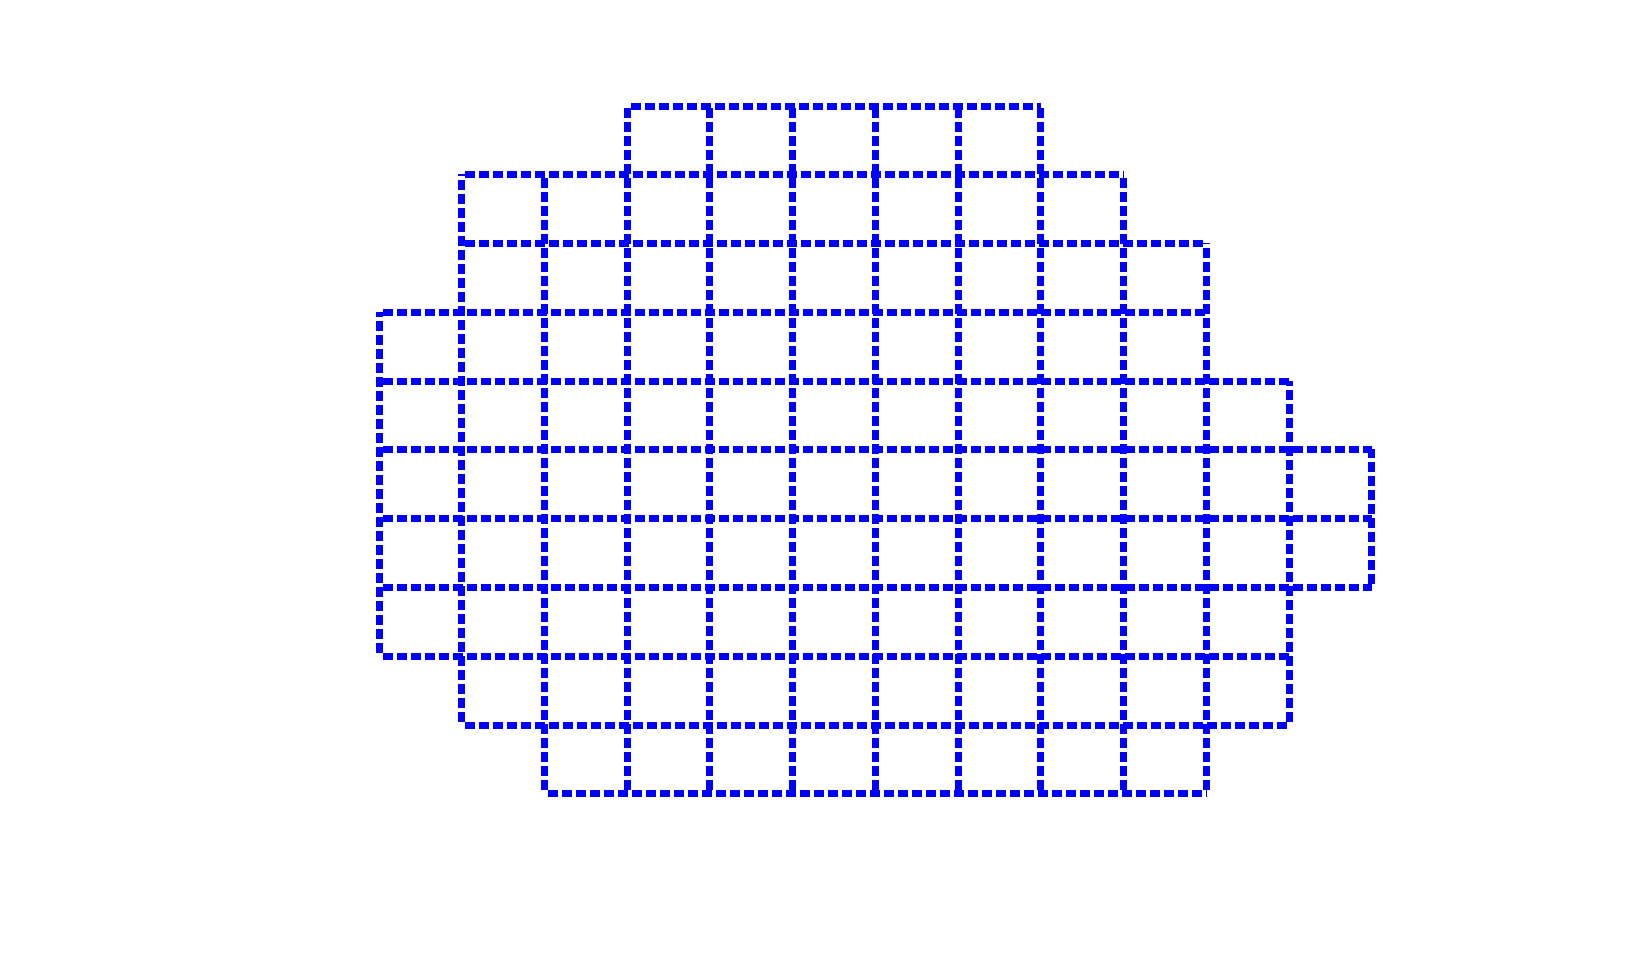
\includegraphics[width=0.3\textwidth]{Chapter3/Figures/OG.png}}\hfill
  \subfloat[][]{
    \label{fig:GridGaussian}\includegraphics[width=0.3\textwidth]{Chapter3/Figures/GG3_80.png}}\hfill
  \subfloat[][]{
    \label{fig:GridBarrel}\includegraphics[width=0.3\textwidth]{Chapter3/Figures/BG3_145.png}}
  \hspace*{\fill}
  \caption[Data space over sampling algorithm]{Data space transformation: \protect\subref{fig:GridOriginal} original synthetic data, \protect\subref{fig:GridGaussian} \acs*{rdgm} deformation, \protect\subref{fig:GridBarrel} \acs*{bd} deformation.}
  \label{fig:DSOS}
\end{figure}

\subsubsection{Feature space (over/under)-sampling}
These strategies are discussed extensively in Sect.~\ref{sec:chp2-sec5}.
%Obviously in these strategies the sampling is performed in feature space.
In the over-sampling approaches, such as \ac{smote} and \ac{ros}, minority samples are selected or synthetically generated to match the number of majority samples.
Under-sampling approaches reject majority samples to match the number of minority samples.
In this research, we tested all the over- and under-sampling methods mentioned in Sect.~\ref{sec:chp2-sec5}, with the value of $k$ set to 3 for \ac{smote}, \ac{ncr}, \ac{nm1}, \ac{nm2}, and \ac{nm3} algorithms.

\subsection{Classification}\label{chp3-subsec6}
In Sect.~\ref{sec:chp2-sec6}, we discussed different single learner and ensemble approaches. 
Among the aforementioned methods, we chose linear (RBF), kernel \ac{svm} and \ac{lda} as single learners, and \ac{gb}, \ac{rf}, and weighted combination as ensembles.
These classifiers are compared with each other in different experiments.
The \ac{rf} classifier is trained in all the experiments up to its maximum length without pruning.
In the initial experiments, the number of \ac{rf} trees is set to 500 while in the later ones the \ac{rf} is trained with 100 trees.
The \ac{gb} classifier is used with an exponential loss function (See Eq.~\ref{eq:exploss}), shrinkage (regularization) parameter of 0.01, and sub-sampling fraction of 0.7. 
The sub-sampling fraction indicates that in each iteration, only 70\% of the training samples are randomly considered.
The optimum regularization and soft margin parameter of the \ac{svm} classifier is set through a grid-search over the validation set. 

Depending on the experiments, different cross-validation approaches (\ac{loocv} or \ac{kcv}) are used as well.
These approaches are explained in the following section along with their corresponding experiments.





%%% Local Variables: 
%%% mode: latex
%%% TeX-master: "../thesis"
%%% End: 
